\chapter{Results and Discussion}

The second step of this work was the analysis of the generated datasets. Thanks to the structure
and the heavy pruning the analysis of these datasets was fast, this allowed us to have a better workflow
without any interruption. We analyzed the data in two ways: a descriptive statistic and an interactive
one.
\paragraph*{Descriptive}
For each dataset, there is a script that plots various statistics using the python libraries
Pandas and Matplotlib. There are two types of output: plots and rankings. 
Plots are useful to understand the trend from a more comprehensive point of view and on a monthly base.  
Rankings are instead used to see the pages/users ordered in a more specific way by one of the
metrics previously computed. 
\paragraph*{Interactive}
This section is still under contruction. We will make an interactive dashboard available online. The idea is
that everyone can change a few parameters and see how the metrics are performing in a personalized
way. To achieve this we uploaded our dataset on a database and thanks to an innovative way to retrieve
data (grapQL) we can display it on a website. 


\section{General statistics}
\paragraph*{Number of reverts in pages}
As we can see in Table \ref{table:pagesmorechains} in the largest part of the pages there are not
any reverts. The filtering of Wikimedia History Dumps removed all the pages with zero reverts. To
compute this field we needed the total number of articles in Wikipedia, a value that is avaiable on
the statistics page of Wikipedia.\footnote{\url{https://en.wikipedia.org/wiki/Special:Statistics}\\
                                            } 
To compute how many pages have 0 reverts we
subtracted the number of pages with at least one revert from the total number of pages.

\begin{table}[H]
    \centering
    \ra{1.2}
    \begin{tabularx}{\columnwidth}{@{}Xrrrr@{}}
        \midrule
        \textbf{n\_reverts} & \textbf{n\_pages\_it} & \textbf{n\_pages\_ca}& \textbf{n\_pages\_en} & \textbf{n\_pages\_es}  \\ \toprule
        0 & 1.296.915& 626,5326 & 4,672,316& 1,411,056\\
        1   & 186,539& 32,233 & 1,272,960& 116,011\\
        2-4 & 122,072& 15,387 & 949,689& 84,324\\
        5-9 & 45,391& 4,791 & 388,839& 35,461\\
        10-99 & 47,833& 3,906 & 472,379& 44,155\\
        100-999 & 4,145& 84& 69,804 & 7113\\

        \bottomrule
    \end{tabularx}
    
    \caption{Number of reverts for Italian, Catalan, English and Spanish Wikipedia. \label{table:pagesmorechains}}
\end{table}

\paragraph*{M}
% qui qui uqi uqi uiq uiqqui qui uqi uqi uiq uiqqui qui uqi uqi uiq uiqqui qui uqi uqi uiq uiqqui qui uqi uqi uiq uiqqui qui uqi uqi uiq uiqqui qui uqi uqi uiq uiqqui qui uqi uqi uiq uiqqui qui uqi uqi uiq uiqqui qui uqi uqi uiq uiq
In this graph, we can see a comparison between M and the total number of reverts done and we can
notice how M had a big growth until 2019 where it remained stable. The fast growth can be
reconducted to the fact that M is calculated from the edit count of the users, so as the years went by the
users got more experienced and then the edit count grew with a direct consequence on M.
\begin{figure}[H]
    \centering
    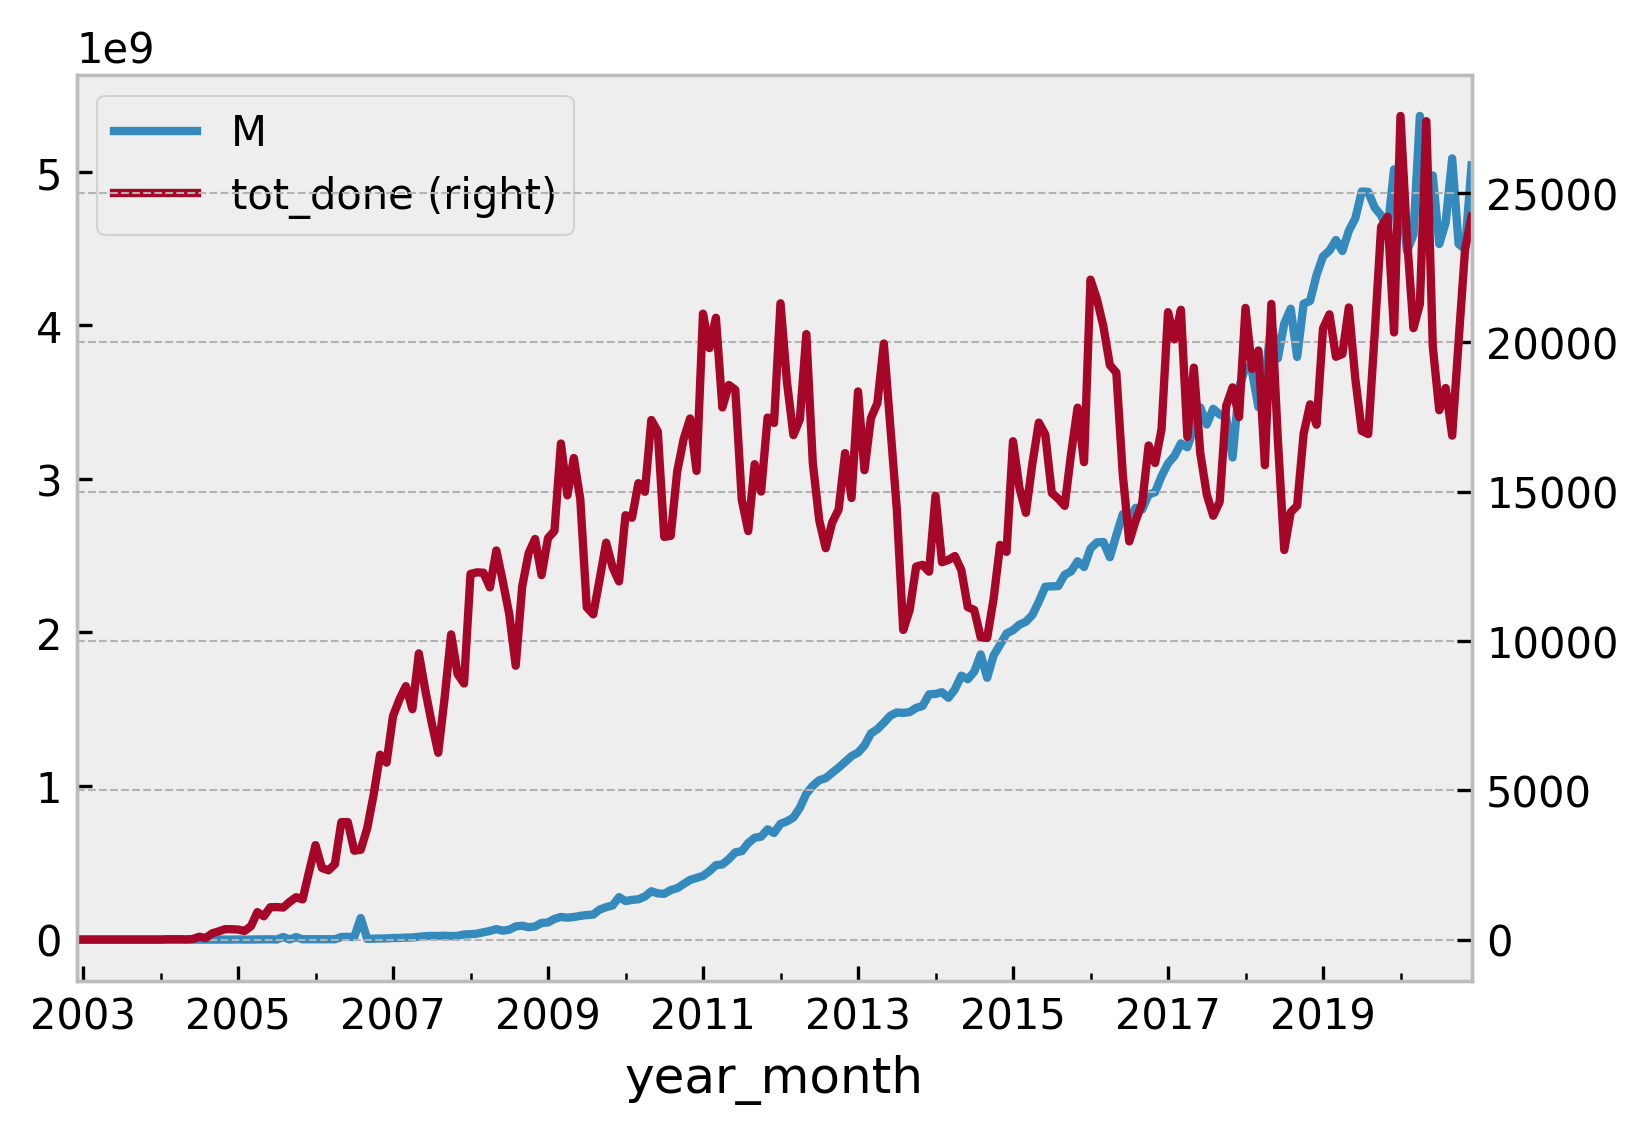
\includegraphics[width=0.6\textwidth]{./chapters/04/assets/Mcompare.png}
    \caption{M compared to the number of Reverts. The values of the total reverts done are represented on the right Y axe.}
    \label{table:mcompare}
\end{figure}
\section{Revert Chains}
Thanks to the analysis of the page chains we can have an overview of an entire Wikipedia in a
language, discovering statistics like the mean length of chains or the longest one. Another aspect
worth investigating was the relationship between solitary reverts and reverts that are in a chain: more
reverts in the chains means more conflicts. In cases like these, combining the data of the other team
members who analyzed the talk pages could be useful to better understand the dynamics. While the chains in
the pages are useful to have a less specific but wider view of the phenomenon, studying the chains a
user joined lets us see if a specific user is involved in many chains and in which pages is more
active. In this sense, we can define different categories of users: the ones who are active just in
some topic or the others who revert on all Wikipedia. \\

Monthly metrics are even more interesting: we can plot the trend of reverts on a page and see if it
is always controversial or just in a specific historical moment related to something that happened
in the world. Plotting the metrics year by year allows us to understand the global activity of the
users on Wikipedia. We can define the lifecycle of a user and see when it is more active, and if
its decrease of revisions is related to a conflict.\\


In Table \ref{table:generalstats} there is an overview of the number of solitary reverts and reverts
that belong to a chain in the Wikipedia of different languages. The ratio between the number of
reverts that are in a chain and the ones that are not is a useful indicator of how much the users
are prone to conflicts. In the Catalan Wikipedia, this ratio is higher than in the ones in Spanish,
Italian, and English; we will explore later in Table \ref{table:morechains} the most conflictual topics.
Further studies about the relationship between the number of reverts and the family of the language could be done.

\begin{table}[H]
    \centering
    \ra{1.2}
    \begin{tabularx}{\columnwidth}{@{}Xrrrrr@{}}
        \midrule
        \textbf{language}& \textbf{revisions} & \textbf{reverts} & \textbf{reverts on edits} & \textbf{reverts in chain} & \textbf{\% in chain} \\ \toprule
        en &1,027,188,756&66,147,314&6.4\%&6,144,948& 10\%\\
        es &136,318,137& 11,539,552&8.4\%& 1,065,618 & 9\% \\
        it &121,362,136& 7,712,039 &6.4\% & 850,020 &  11\% \\
        ca &27,657,030& 355,251 & 1.3\%& 56,280 & 15\% \\
    
        \bottomrule
    \end{tabularx}
    
    \caption{Number of reverts in chains in Wikipedia in Spanish, Italian, and Catalan. \label{table:generalstats}}
\end{table}


\subsection{Revert chains analysis by page}
In Table \ref{table:morechains}, the pages are ranked by the number of chains in Italian, Catalan,
and Spanish. In the Italian one six out of ten pages were football-related while in the catalan one
we can see, as expected, a stronger territorial belonging, the Spanish ranking tells us that the
main part of Spanish Wikipedia users are from Latin America and that they are interested in
football. 
\begin{table}[H]
    \centering
    \ra{1.2}
    \begin{tabularx}{\columnwidth}{@{}Xll|ll|ll@{}}
        \midrule
        \textbf{id} & \textbf{title it} & \textbf{chains}& \textbf{title ca} & \textbf{chains}&\textbf{title es} & \textbf{chains} \\ \toprule
        1 & Serie A & 195  & Barcelona & 68 & Club América & 222\\
        2 & Juventus FC & 190  & FC Barcelona & 33 & Deporte en Argentina & 218\\
        3 & Matteo Renzi & 179  & Catalunya & 30 & Club Universitario & 213\\
        4 & AS Roma & 176  &País Valencià& 26 & Club Guadalajara & 211\\
        5 & Personale WWE & 167  &Marc Márquez i Alentà & 22 & América Latina & 185\\
        6 & SSC Napoli & 162  & Mireia Belmonte i García& 22 & Club Alianza Lima & 179\\
        7 & Inter  & 162  &Girona & 20 & Idioma español & 171\\
        8 & Roma & 154 & Rafael Nadal i Parera & 19 & Juventus de Turín & 162\\
        9 & Tiziano Ferro & 141 & Oriol Junqueras i Vies& 17 & Ecuador & 160\\
        10 & Gianluigi Buffon & 137  &Català & 16 & Bogotá & 159\\
        
         \bottomrule
    \end{tabularx}
    
    \caption{Top 10 pages by number of revert chains in the Italian, Catalan and Spanish Wikipedia. \label{table:morechains}}
\end{table}


In the analysis of the longest chain, the scenario we face is different. The top topics are not
sports but cinema, music and literature for Italian. But here the most fascinating things happen on
the Catalan Wikipedia: we can see how the longest chains are all related to Navarra, doing a more
specific research we can see that it is all related to the language used to identify cities, this is
probably vandalism from some Spanish user who wanted to suppress the Basque language. These metrics
can be used to detect problems between experienced users but can let some sociopolitical
issue inside a place with linguistic minorities emerge.
\begin{table}[H]
    \centering
    \ra{1.2}
    \begin{tabularx}{\columnwidth}{@{}Xll|ll|ll@{}}
        \midrule
        \textbf{id} & \textbf{title it} & \textbf{longest}& \textbf{title ca} & \textbf{longest} & \textbf{title es} & \textbf{longest} \\ \toprule
        1 & Pino Rauti  & 114  & Roncal-Salazar & 81 & Alan  Jackson & 178\\
        2 & Carlos Tévez & 66  & Tractat  d'Utrecht & 80 & A & 172\\
        3 & Rogue  One & 64  & Gazteluberri & 76 & Consejo  Mundial  de  Boxeo & 140\\
        4 & Rocky  Marciano & 64  &Comarca  de  Sangüesa& 71 & Guerra  anglo-española  (1625-1630) & 140\\
        5 & Poeta  urbano & 58  &Comarca  d'Aoiz & 69 & Guerra  de  la  Independencia  Española& 137\\
        6 & Paradisi  per  illusi & 55  & Comarca  de  Lumbier& 69 & Guerra  anglo-española  (1585-1604) & 121\\
        7 & Kuromajo-san  ga  toru!  & 53  &Riu  Gor & 53 & Independencia  de  la  República  Dominicana & 107\\
        8 & Matt  Dillo & 52 & Tudela & 51 & Kreutzberger & 100\\
        9 & Aletheia  (album) & 52 & Igúzquiza& 50 & Dalas  Review & 99\\
        10 & Franz  Kafka & 51  &Untziti & 48 & Bastille & 96\\


         \bottomrule
    \end{tabularx}
    
    \caption{Pages sorted by longest chains. \label{table:longestchain}}
\end{table}


\paragraph*{Monthly}
By analyzing the trend (Fig \ref{fig:chainsuser}) of the page (Barcelona in Catalan) we can clearly
see that even if there are a lot of chains the controversiality metric G grows mainly on one
occasion; the reason is that in the one where more experienced users are involved this metric is useful
to detect conflicts between them.
\begin{figure}[H]
    \centering
    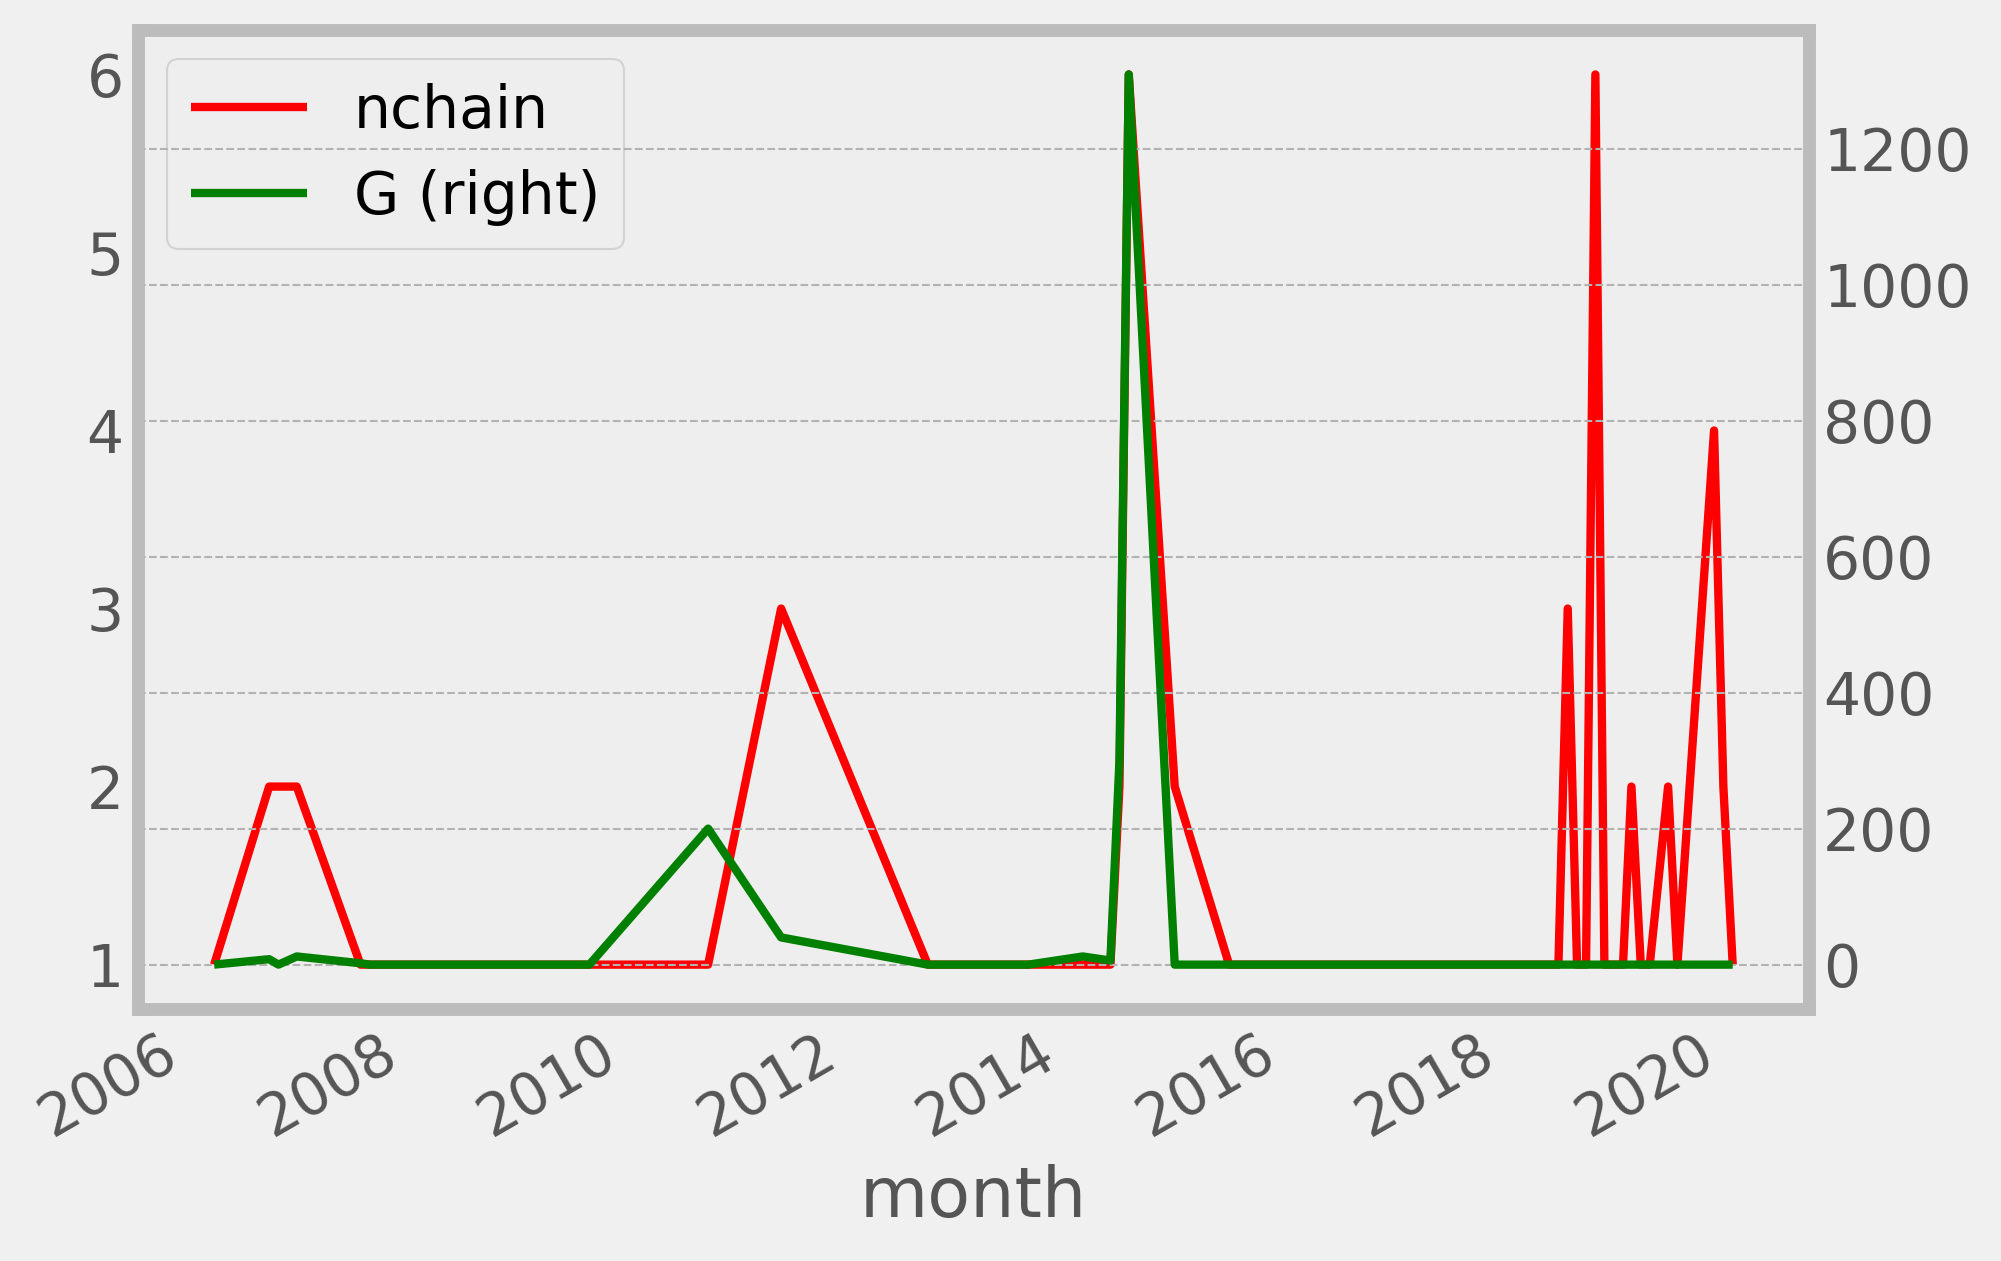
\includegraphics[width=0.7\textwidth]{./chapters/04/assets/chains_page.png}
    \caption{G and the number of chains for the Barcelona page in Catalan. The value of G is represented on the right Y axe.}
    \label{fig:chainsuser}
\end{figure}

\subsection{Revert chains analysis by user}
In Table \ref{table:userinchains} the data about the number of users was aggregated by the number of
joined chaines, we can see that most of the users are not involed in chains. In the Italian Wikipedia
more than 11\% of users are involved in at least one chain versus the less than 4\% of the English Wikipedia.

\begin{table}[H]
    \centering
    \ra{1.2}
    \begin{tabularx}{\columnwidth}{@{}Xrrr@{}}
        \midrule
        \textbf{language}& \textbf{users} & \textbf{users in chains} & \textbf{ratio} \\ \toprule
        en &41,840,255&1,569,240&3.7\%\\
        es &6,268,217& 283,914&4.5\% \\
        it &2,141,529& 248,646 &11.6\% \\
        ca &391,272& 12,565 & 3.2\% \\
    
        \bottomrule
    \end{tabularx}
    
    \caption{Number of users in chains in Wikipedia in Spanish, Italian, and Catalan. \label{table:userinchains}}
\end{table}

Table \ref{table:usersmorechains} contains the data concerning the number of users grouped by the number of chains joined.

\begin{table}[H]
    \centering
    \ra{1.2}
    \begin{tabularx}{\columnwidth}{@{}Xrrrr@{}}
        \midrule
        \textbf{n\_chains\_joined} & \textbf{n\_users\_it} & \textbf{n\_users\_ca}& \textbf{n\_users\_en} & \textbf{n\_users\_es}  \\ \toprule
        0 & 1,892,837 & 378,697& 40.270.206& 5.985.304\\
        1   & 211,746 & 10,500 & 1,281,670& 246,015\\
        2-4 & 29,685  & 1,548 & 217,140& 30,010\\
        5-9 & 4,066   & 231 & 37,448& 4,331\\
        10-99 & 2,672 & 249 & 28,734& 2,999\\
        100-999 & 477& 37  & 4'247 & 558\\
        \bottomrule
    \end{tabularx}
    \caption{Number of users that joined chains for Italian, Catalan, English, and Spanish Wikipedia.\label{table:usersmorechains}}
\end{table}
% Table \ref{table:mean} ranks the users by the mean length of the chains they joined. All of them are anonymous users.
% The longest chains are usually about details (like, for example, the number of championships won by Juventus) that are
% continuously modified until the vandal is blocked.

% \begin{table}[H]
%     \centering
%     \ra{1.2}
%     \begin{tabularx}{\columnwidth}{@{}Xllll@{}}
%         \midrule
%         \textbf{id}& \textbf{user} & \textbf{nchains} & \textbf{mean}& \textbf{nrevert}  \\ \toprule
%         1 & 95.20.240.x & 7  & 60.4 & 423 \\
%         2 & 95.20.242.x & 1  & 51.0 & 51  \\
%         3 & 37.11.145.x & 14  & 51.0 & 714  \\
%         4 & 95.20.249.x & 14  & 51.0 & 714  \\
%         5 & 83.49.253.x & 1  & 47.0 & 47 \\
        
%          \bottomrule
%     \end{tabularx}
    
%     \caption{User sorted by mean length of the chains joined \label{table:mean}}
% \end{table}

% It is also possible to see on which pages a given user joins more revert wars. Table
% \ref{table:pagesuser}  represents the pages on which the user, let us call him Juan, got involved in more chains in The Catalan
% Wikipedia. In this example, Juan is mainly interested in Catalan famous people
% like sportsmen and writers.

% \begin{table}[H]
%     \centering
%     \ra{1.2}
%     \begin{tabularx}{\columnwidth}{@{}Xllll@{}}
%         \midrule
%         \textbf{id}& \textbf{user} & \textbf{nchains}  \\ \toprule
%         1 & Marc Márquez i Alentà & 14  \\
%         2 & Barcelona & 9   \\
%         3 & Jocs Olímpics d'estiu de 1992 & 7   \\
%         4 & Rafael Nadal i Parera & 6  \\
%         5 & Catalunya &  6 \\
%         6 & Lliga de Campions de la UEFA	 &  6 \\
%         7 & Quim Monzó &  6 \\
%         8 & Polseres vermelles &  6 \\
%         9 & Jordi Sànchez i Zaragoza &  6 \\
%         10 & Alfons Arús i Leita &  6\\

%          \bottomrule
%     \end{tabularx}
    
%     \caption{Top 10 pages by number of chain of Juan. \label{table:pagesuser}}
% \end{table}

\clearpage
\paragraph*{monthly}
Given a user we can draw its revert chain activity. 
\begin{figure}[H]
    \centering
    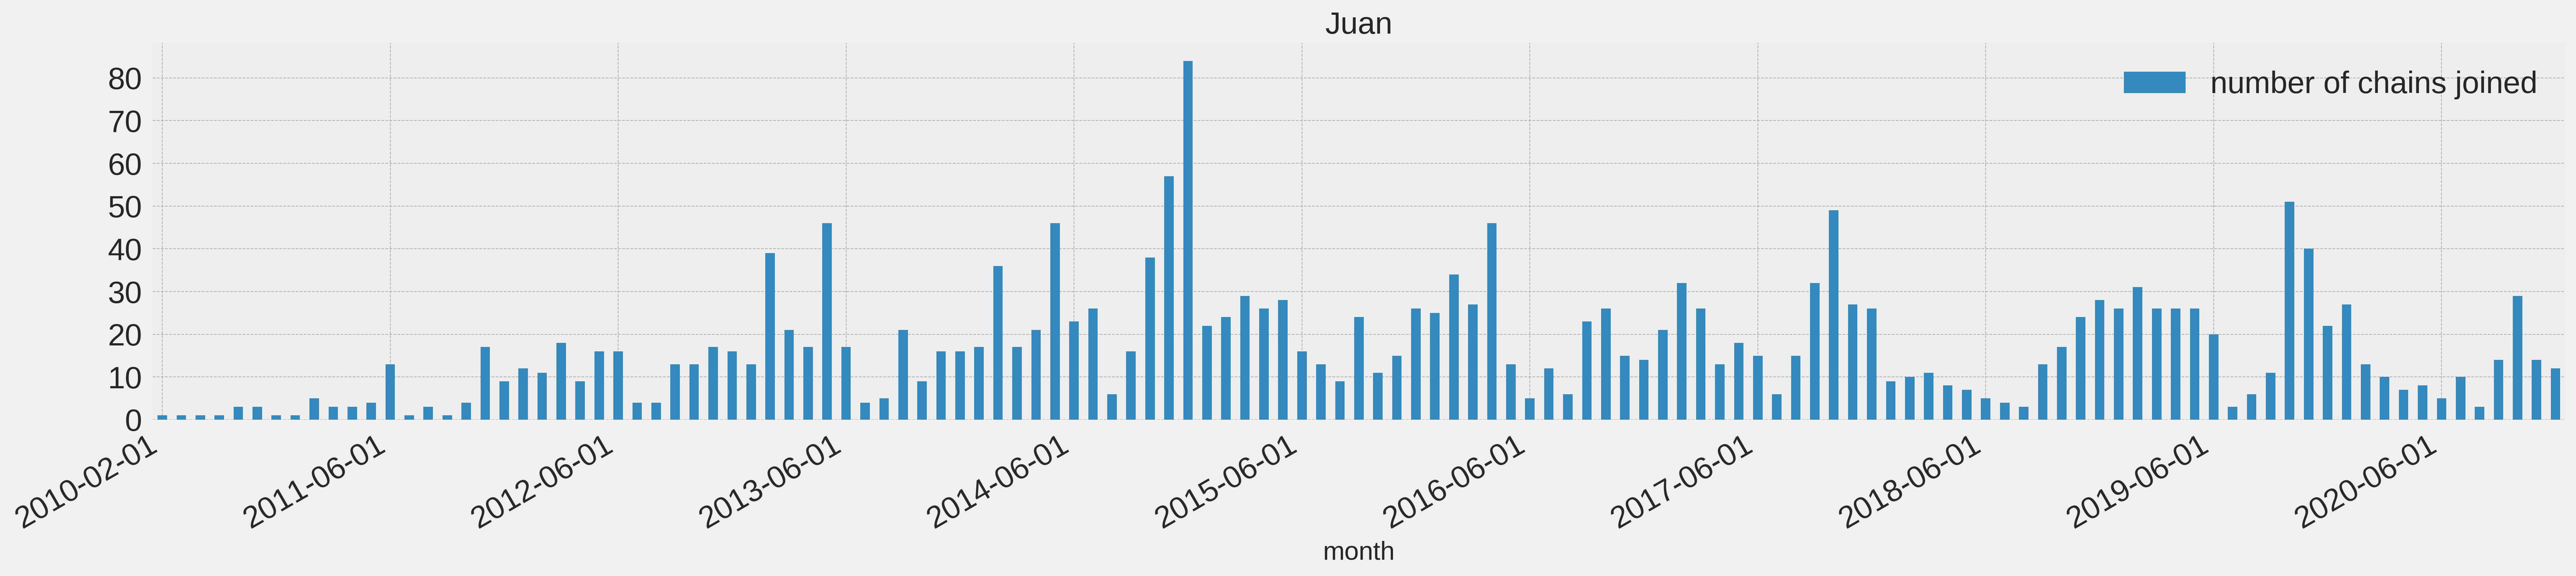
\includegraphics[width=\textwidth]{./chapters/04/assets/chains_user_month.png}
    \caption{Number of chains of an anonymized user by month.}
    \label{fig:chainsusermonth}
\end{figure}




\section{User group analysis}
From the analysis of the groups, we can define different rankings of pages using the number of
reverts of each group. Given a page, we can plot the trend of the edits by group and detect the
pages in which the admins are more active in making reverts. We can say from which category a given user
is the target of reverts and the ratio between made and received reverts. Such a deep analysis of
this data can be done, that is the reason why it is available to everyone who needs it. 

Here are some numbers about the users in different languages, users who have performed an action in
the last 30 days are considered active:
\begin{table}[H]
    \centering
    \ra{1.2}
    \begin{tabularx}{\columnwidth}{@{}Xrrr@{}}
        \midrule
        \textbf{len}& \textbf{registered} & \textbf{admin}& \textbf{active}  \\ \toprule
        en& 41,825,139& 1,089& 127,566  \\
        es & 6,266,812 & 69 & 16,143   \\
        it & 2,140,498 & 114 & 8,208\\
        ca & 391,067 & 22 & 1,180   \\
     

         \bottomrule
    \end{tabularx}
    
    \caption{Number of users by group. \label{table:statsuser}}
\end{table}

\subsection{User activity by group }
For privacy reasons we can only display aggregated data about users. This data is useful to
understand the general trends a Wikipedia in a language is following. The data is divided by user category, therefore we
can draw conclusions about the influence of the different groups in each language. 
\paragraph*{Mutual reverts with admins}
In Table \ref{table:mutadmbin}
is displayed the number of users that are in a mutual revert with admin and the number of them. 

\begin{table}[H]
    \centering
    \ra{1.2}
    \begin{tabularx}{\columnwidth}{@{}Xrrrr@{}}
        \midrule
        \textbf{mut\_adm} & \textbf{n\_users\_it} & \textbf{n\_users\_ca}& \textbf{n\_users\_en} & \textbf{n\_users\_es}  \\ \toprule
        0 & 2,098,014& 388,453 & 41,490,742& 6,245,755\\
        1   & 43,515& 2720 & 342402& 23104\\
        2-4 & 1,300& 91 & 7103& 358\\
        5-9 & 0& 0 & 8 & 0\\
     
        \bottomrule
    \end{tabularx}
    
    \caption{Number of mutual reverts with admin for Italian, Catalan, English, and Spanish Wikipedia. \label{table:mutadmbin}}
\end{table}
\clearpage
\paragraph*{Reverts from a group to another}
In Fig \ref{fig:compare} we can see how the influence of the admins is higher in the Italian
Wikipedia than in the Spanish one. All the spikes we can see in Spanish and Catalan Wikipedias are due to the
seasonality of the user activity: every year during the summer there is a decrease in the edits and
therefore of the reverts. In Catalan, these trends are more visible, and we can see that the number of
reverts made by admin towards registered users is similar to the ones done by registered toward
registered, unlike in the Italian and Spanish cases. 
\begin{figure}[H]
    \centering
    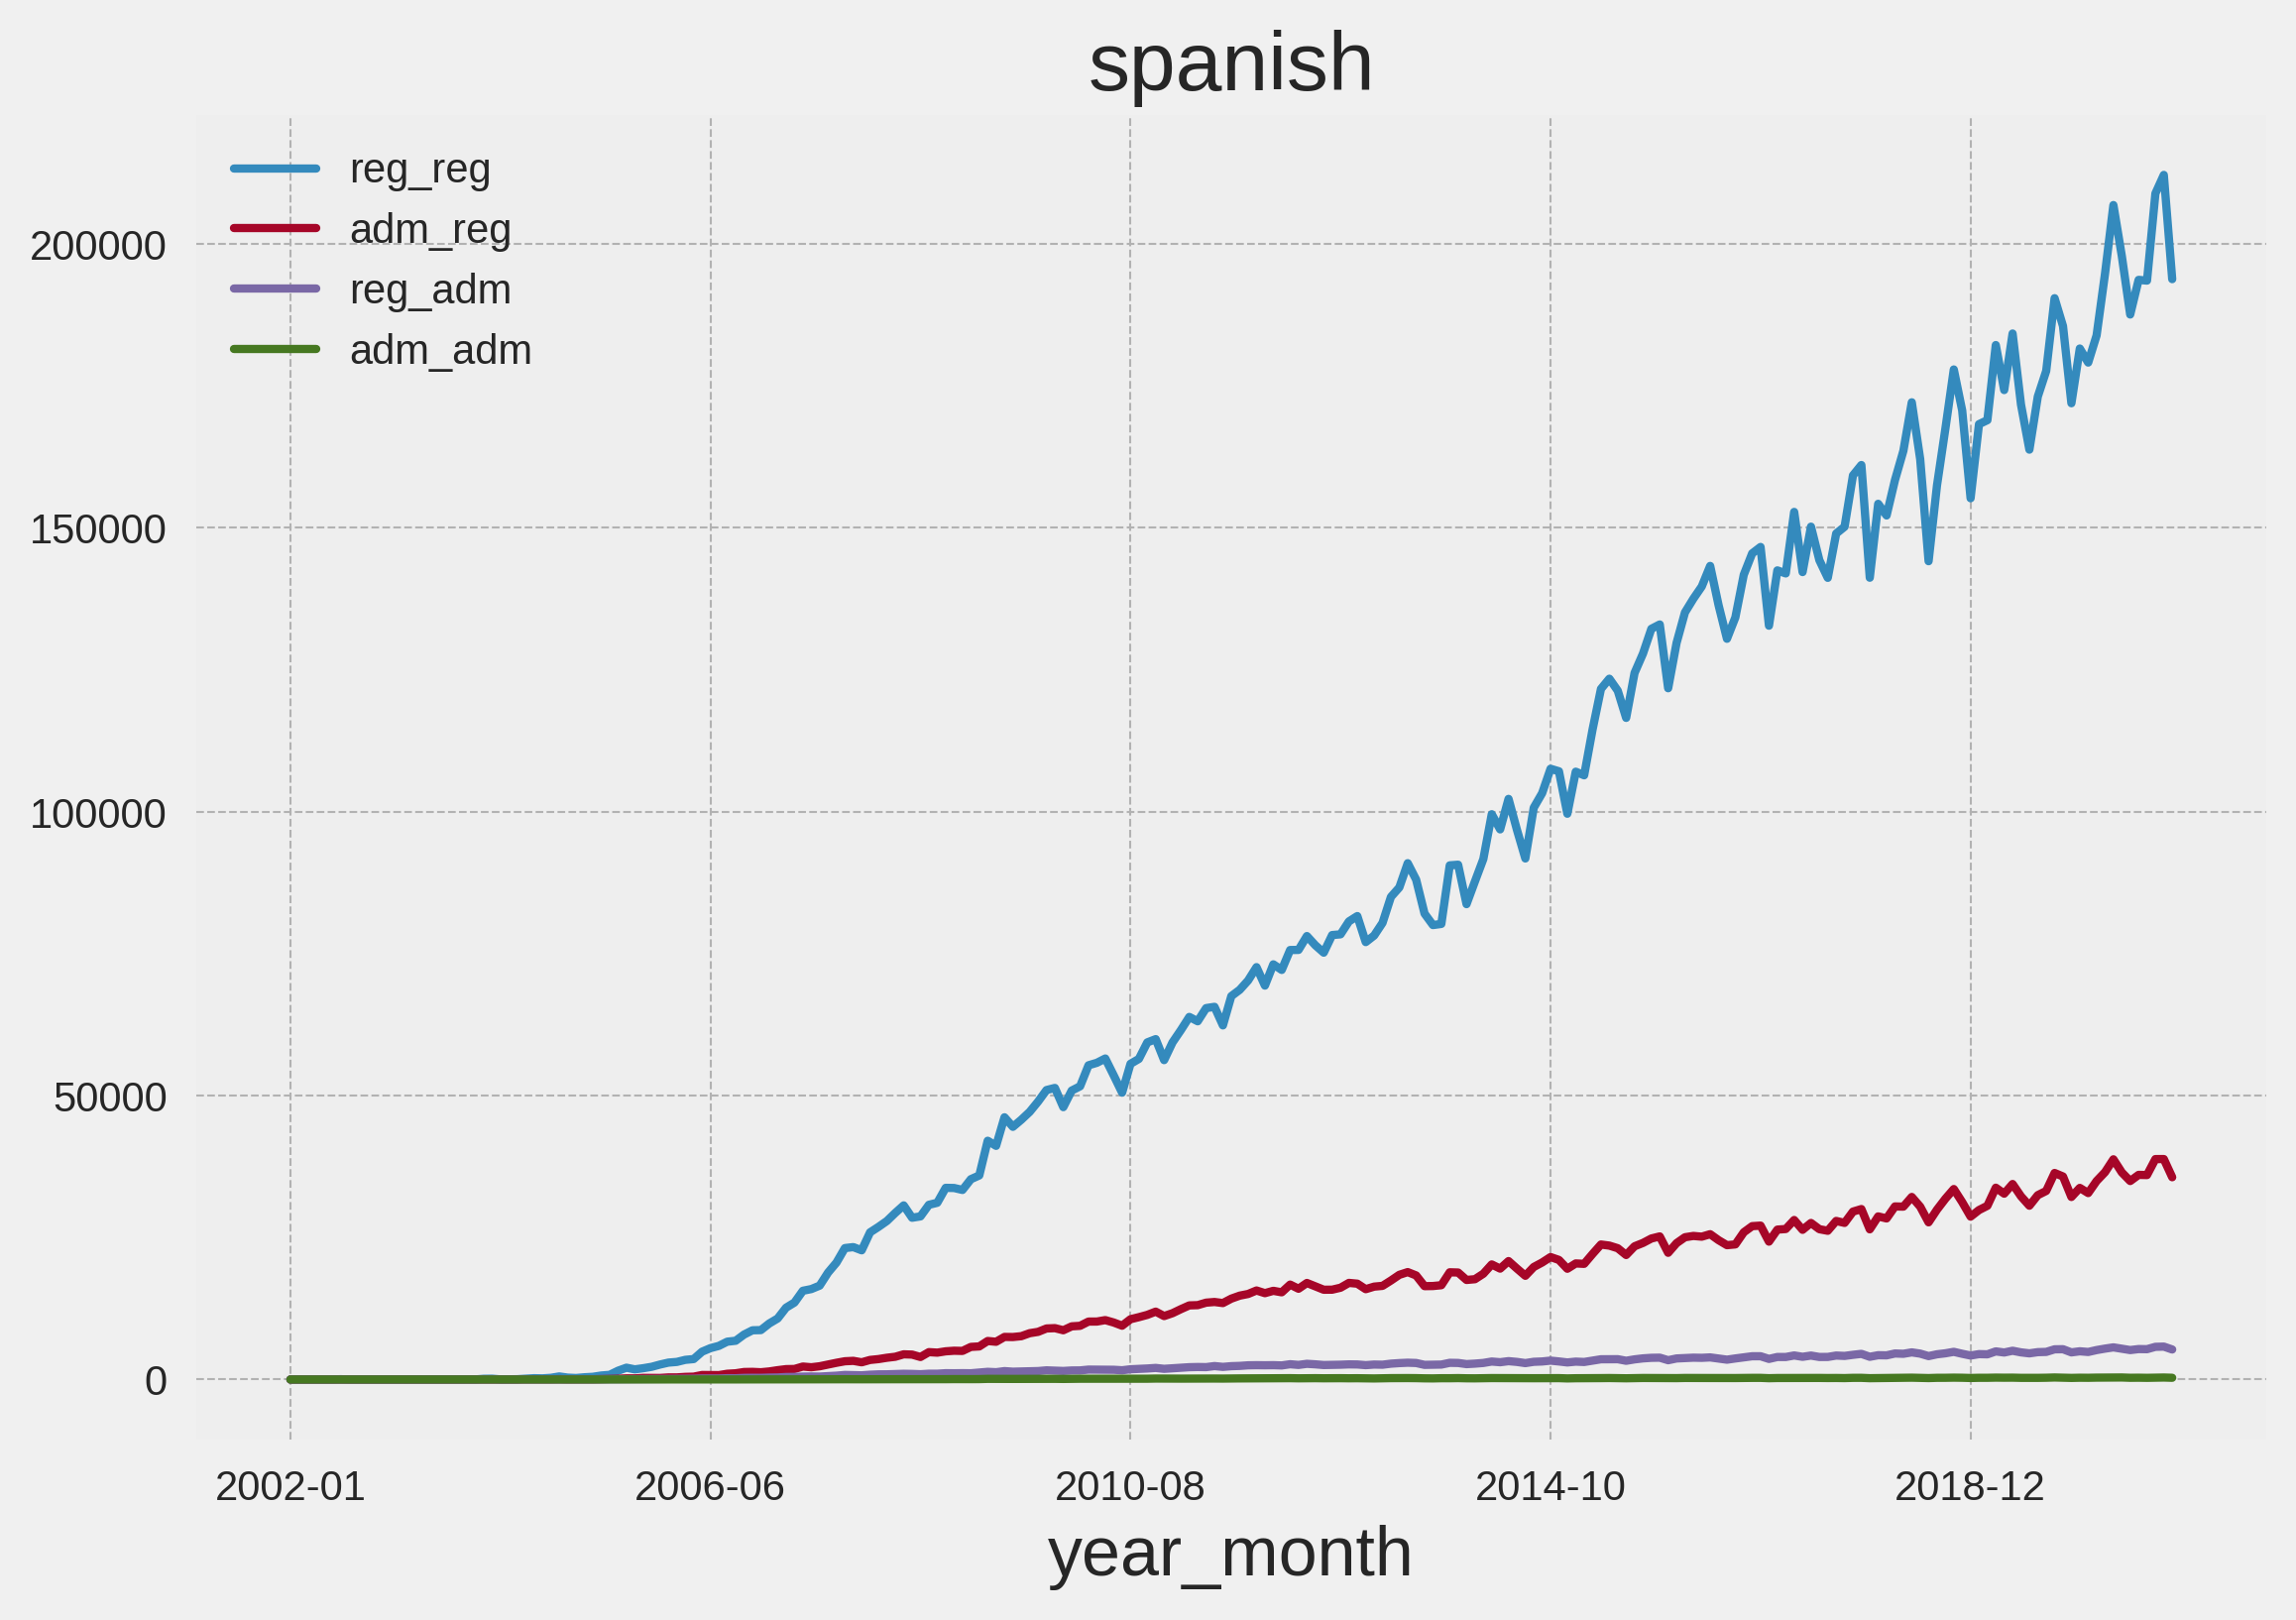
\includegraphics[width=0.6\textwidth]{./chapters/04/assets/admin_es.png}
    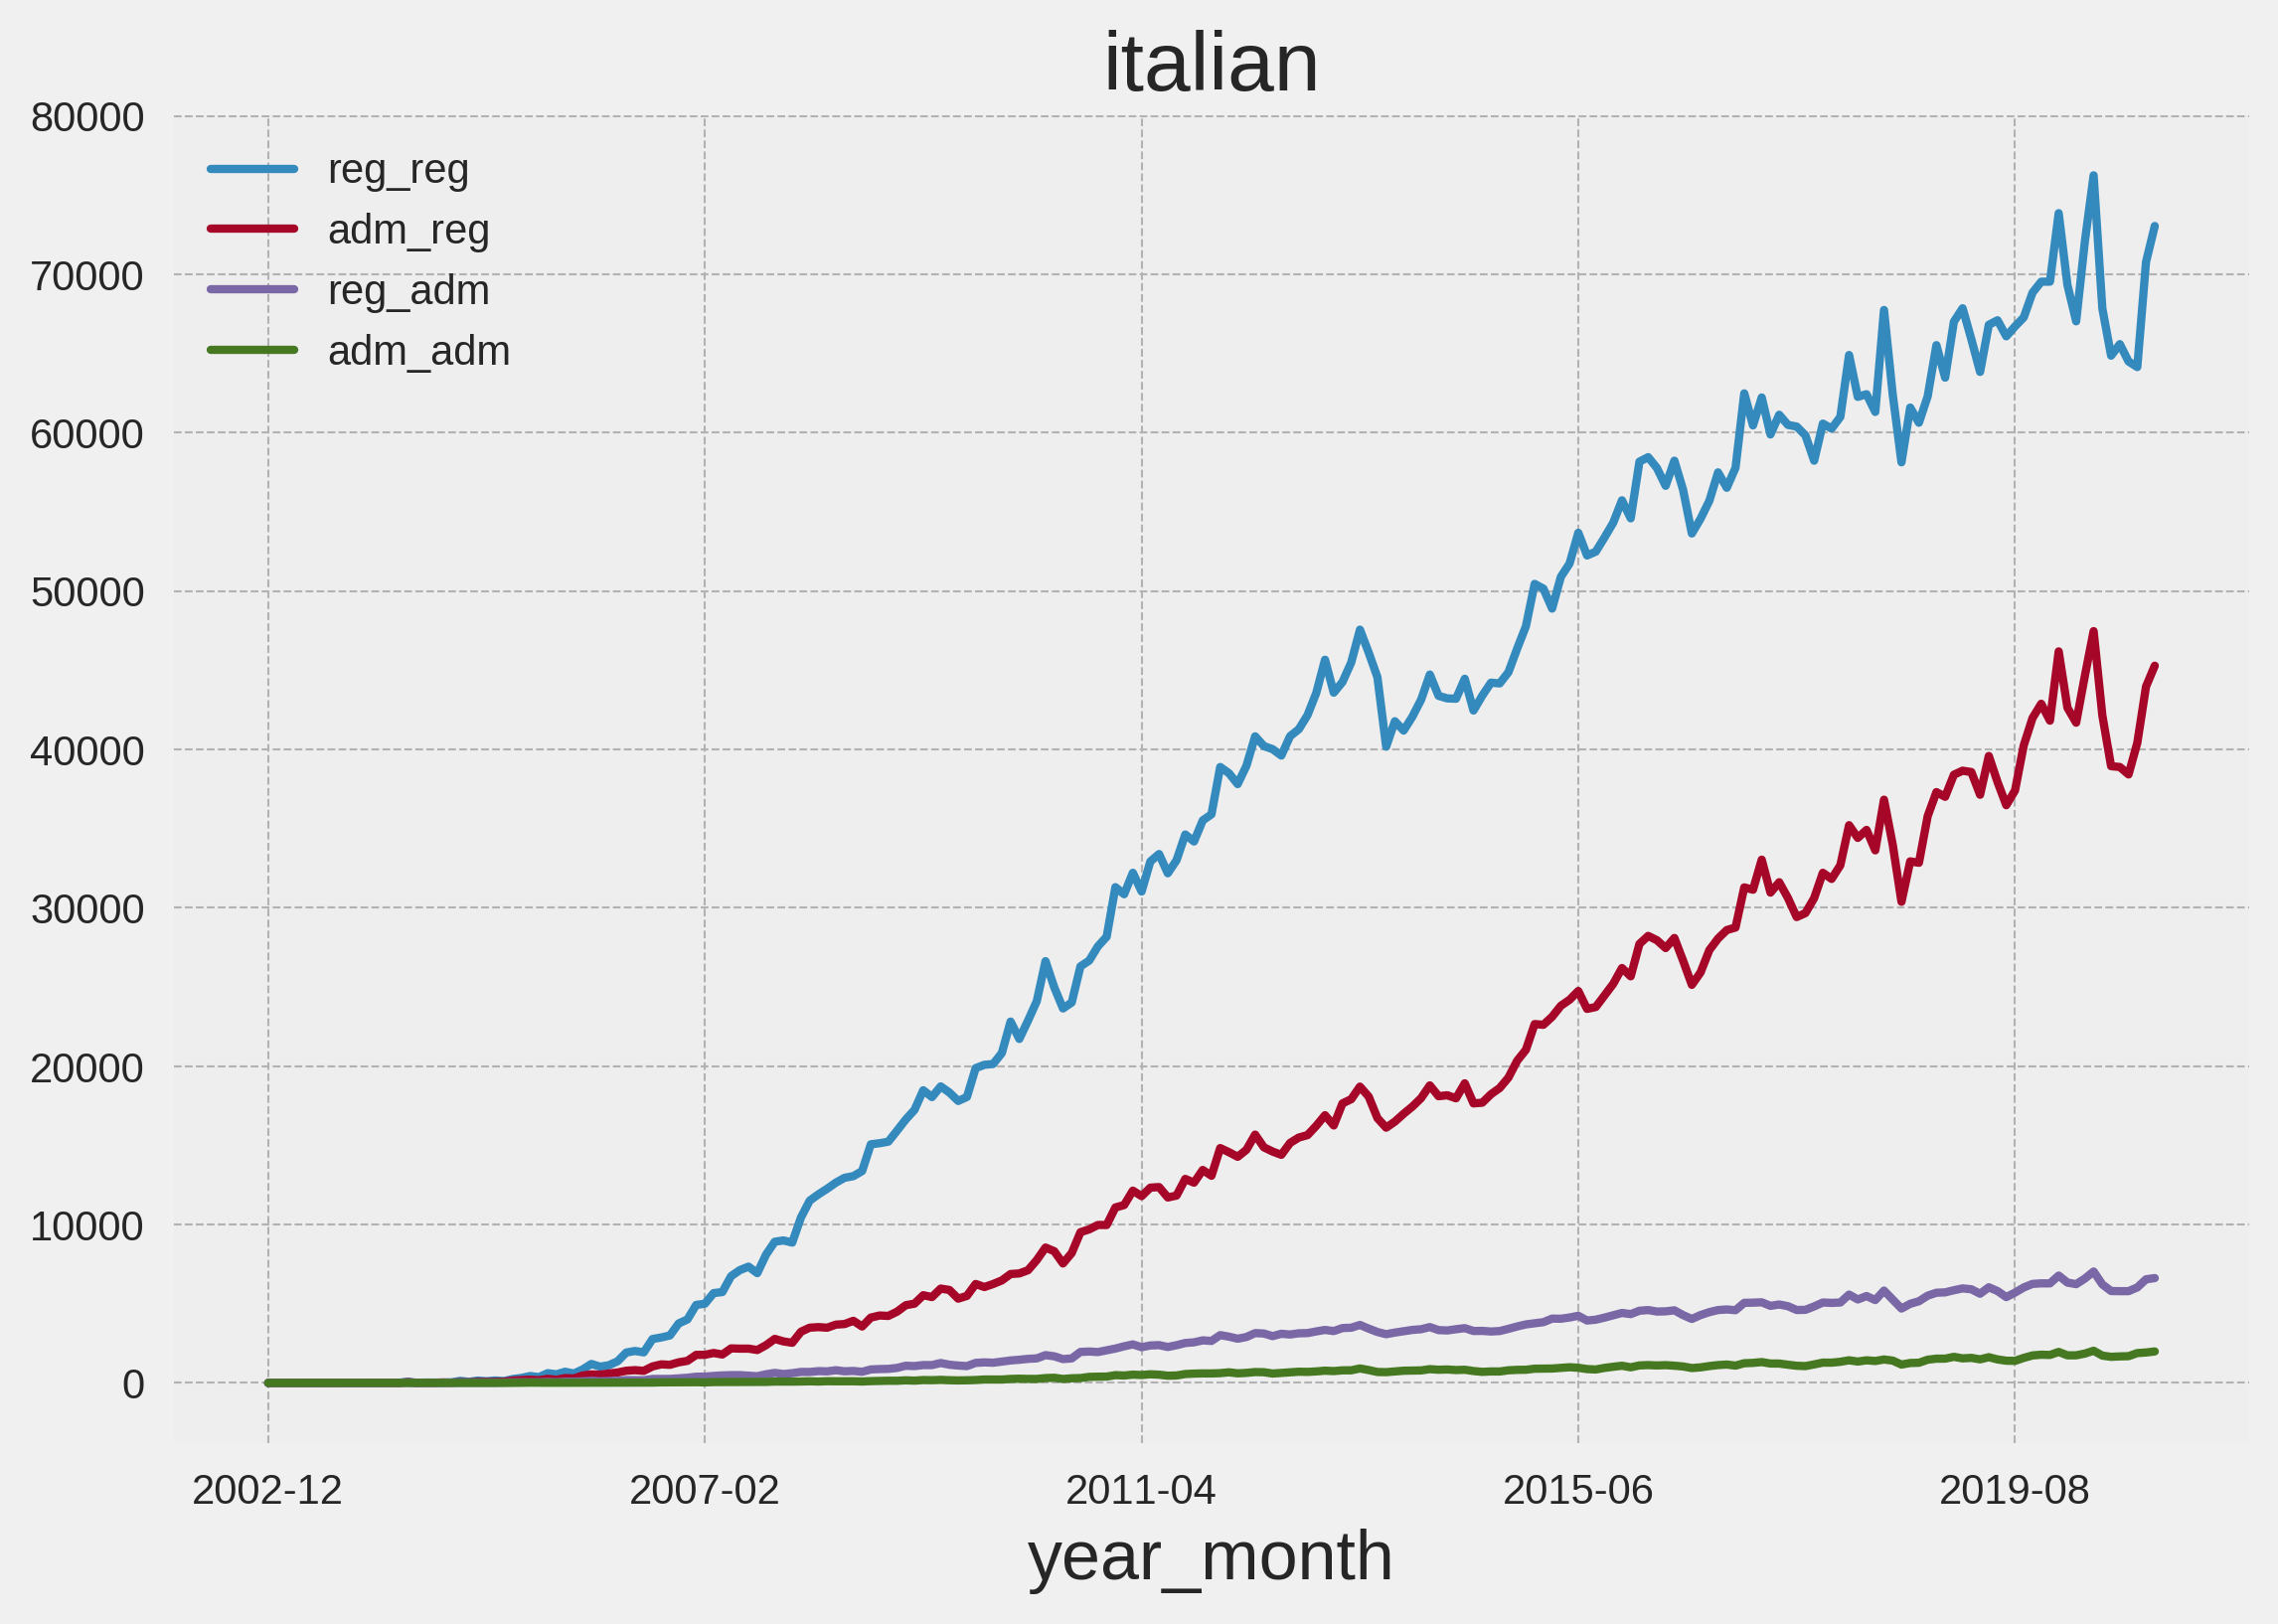
\includegraphics[width=0.6\textwidth]{./chapters/04/assets/admin_it.png}
    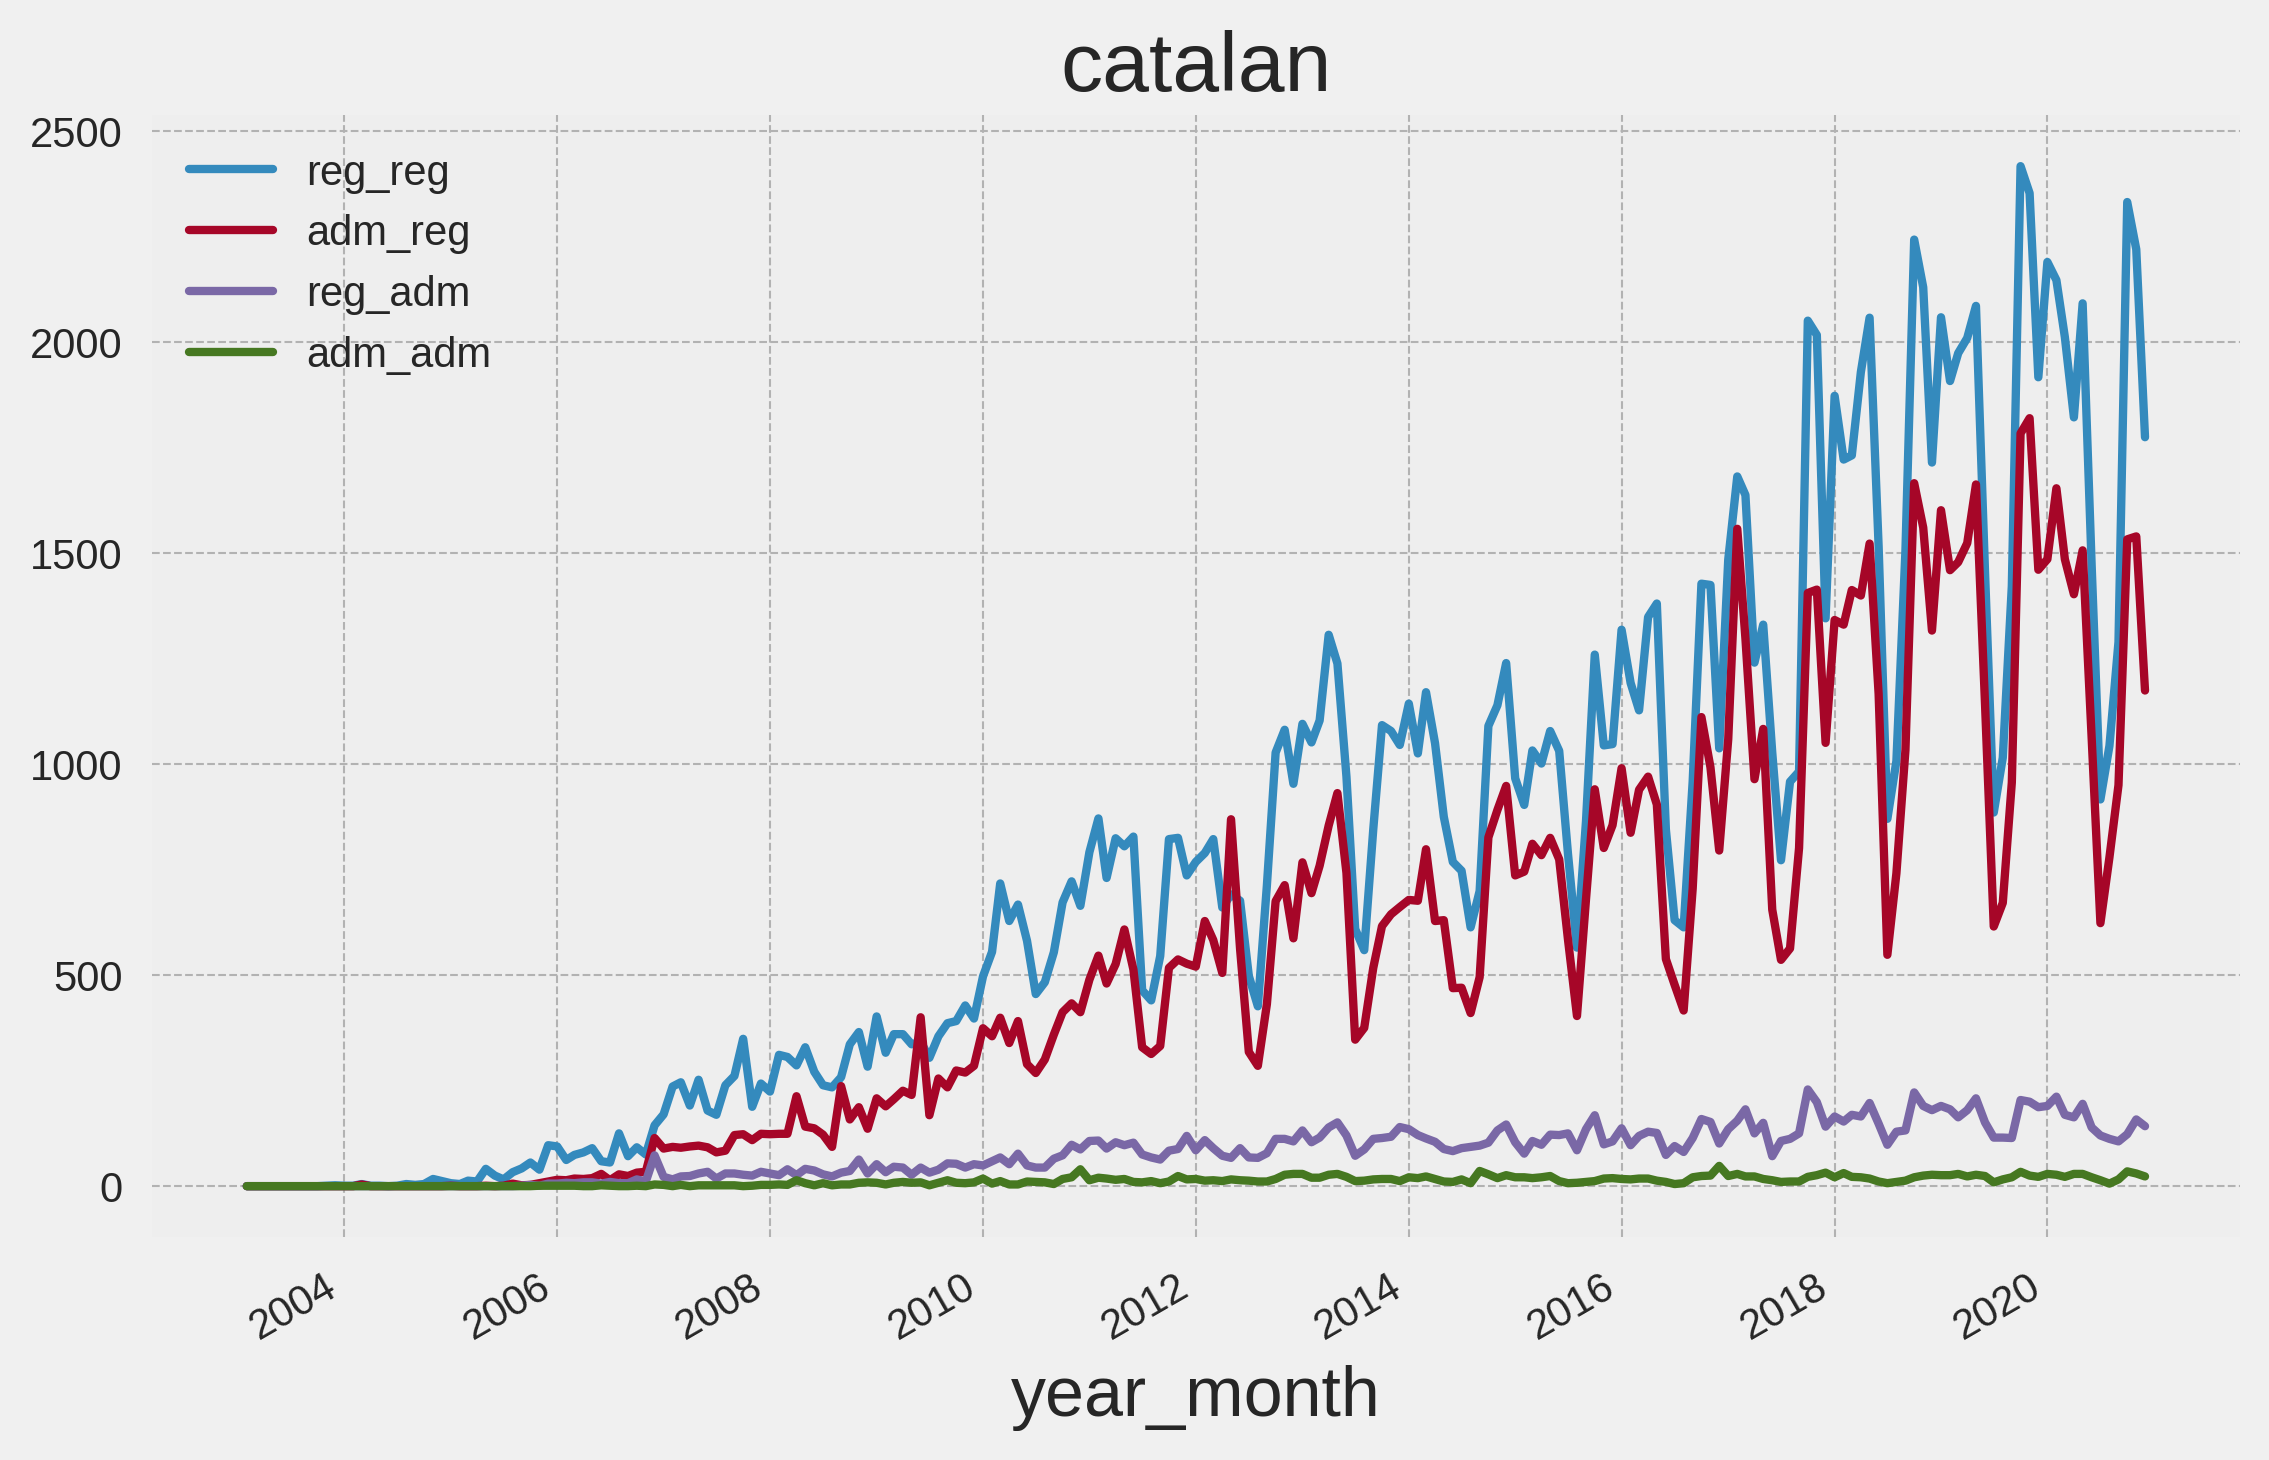
\includegraphics[width=0.6\textwidth]{./chapters/04/assets/admin_ca.png}
    \caption{Number of reverts done divided by group.}
    \label{fig:compare}
\end{figure}


\paragraph*{Reverts made and received}
The plots represent, for Italian, Catalan and Spanish, the number of reverts done and received by
each category; we can see how the behaviour of the users changes with the language especially
towards anonymous users. The Italian and the Spanish trends on done reverts are similar, but the share of
the reverts of the admin in the received ones is very different. In Italy, the received reverts are
equally divided between anonymous and registered.  
\begin{figure}[H]
    \centering
    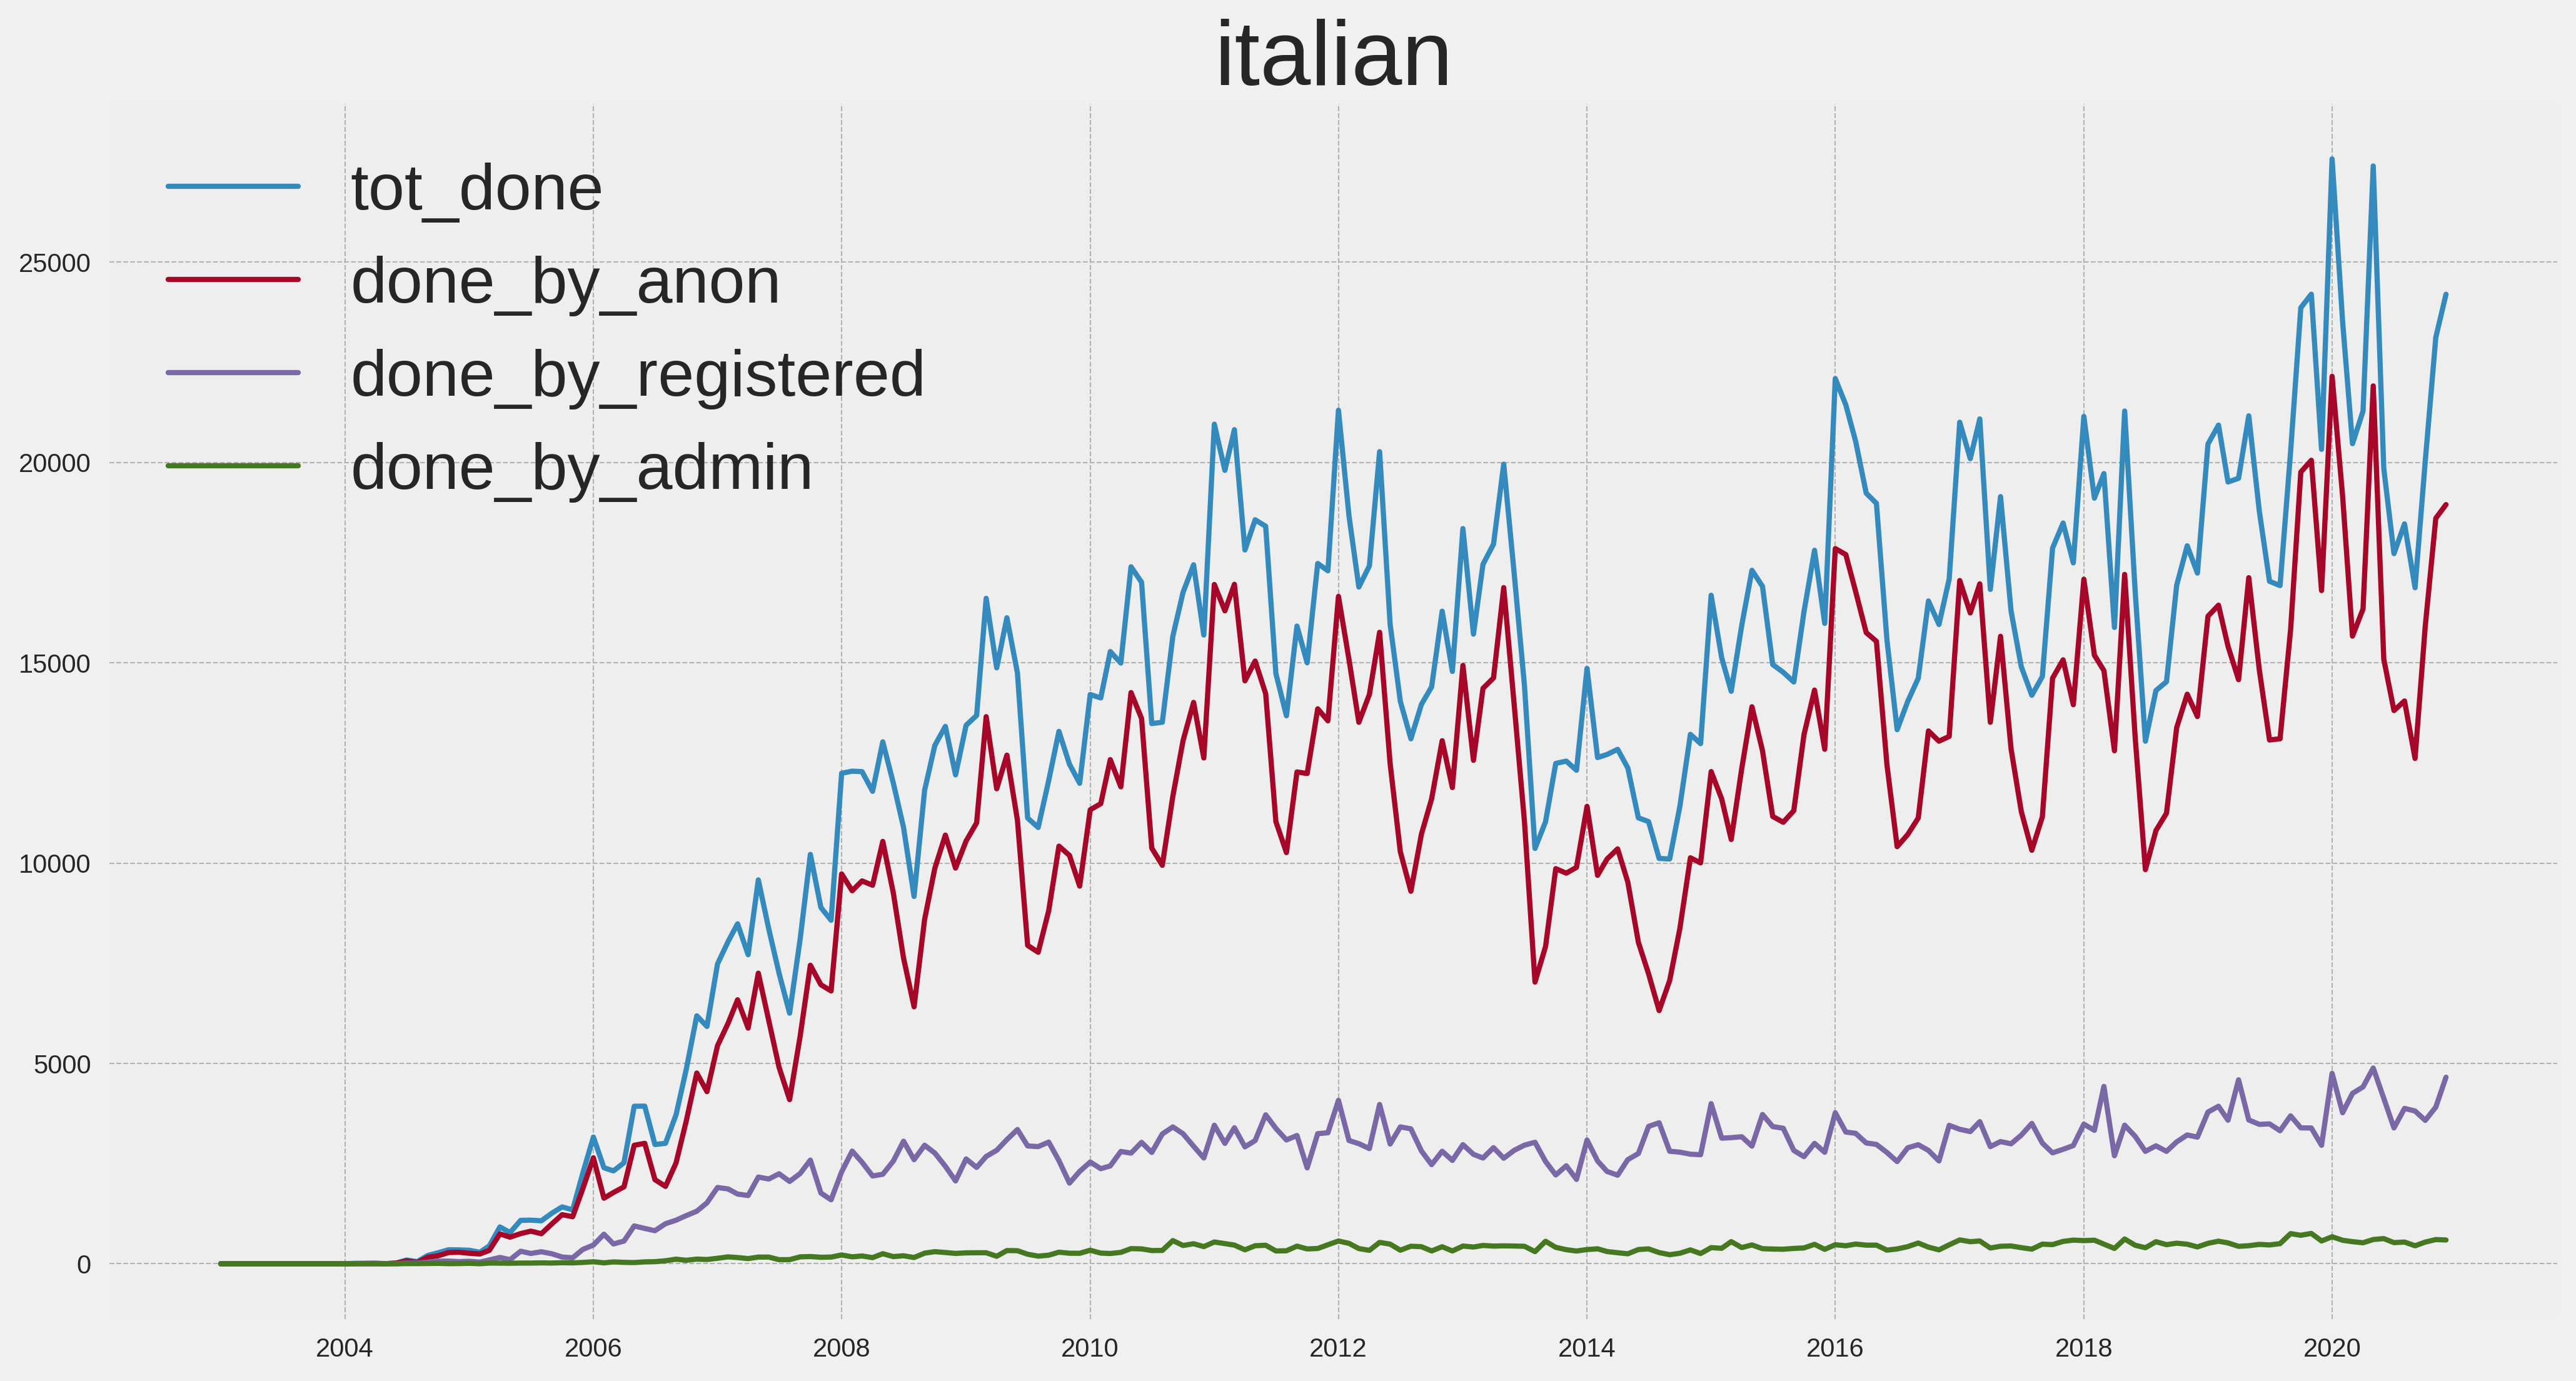
\includegraphics[width=0.49\textwidth]{./chapters/04/assets/revert_done_it.png}
    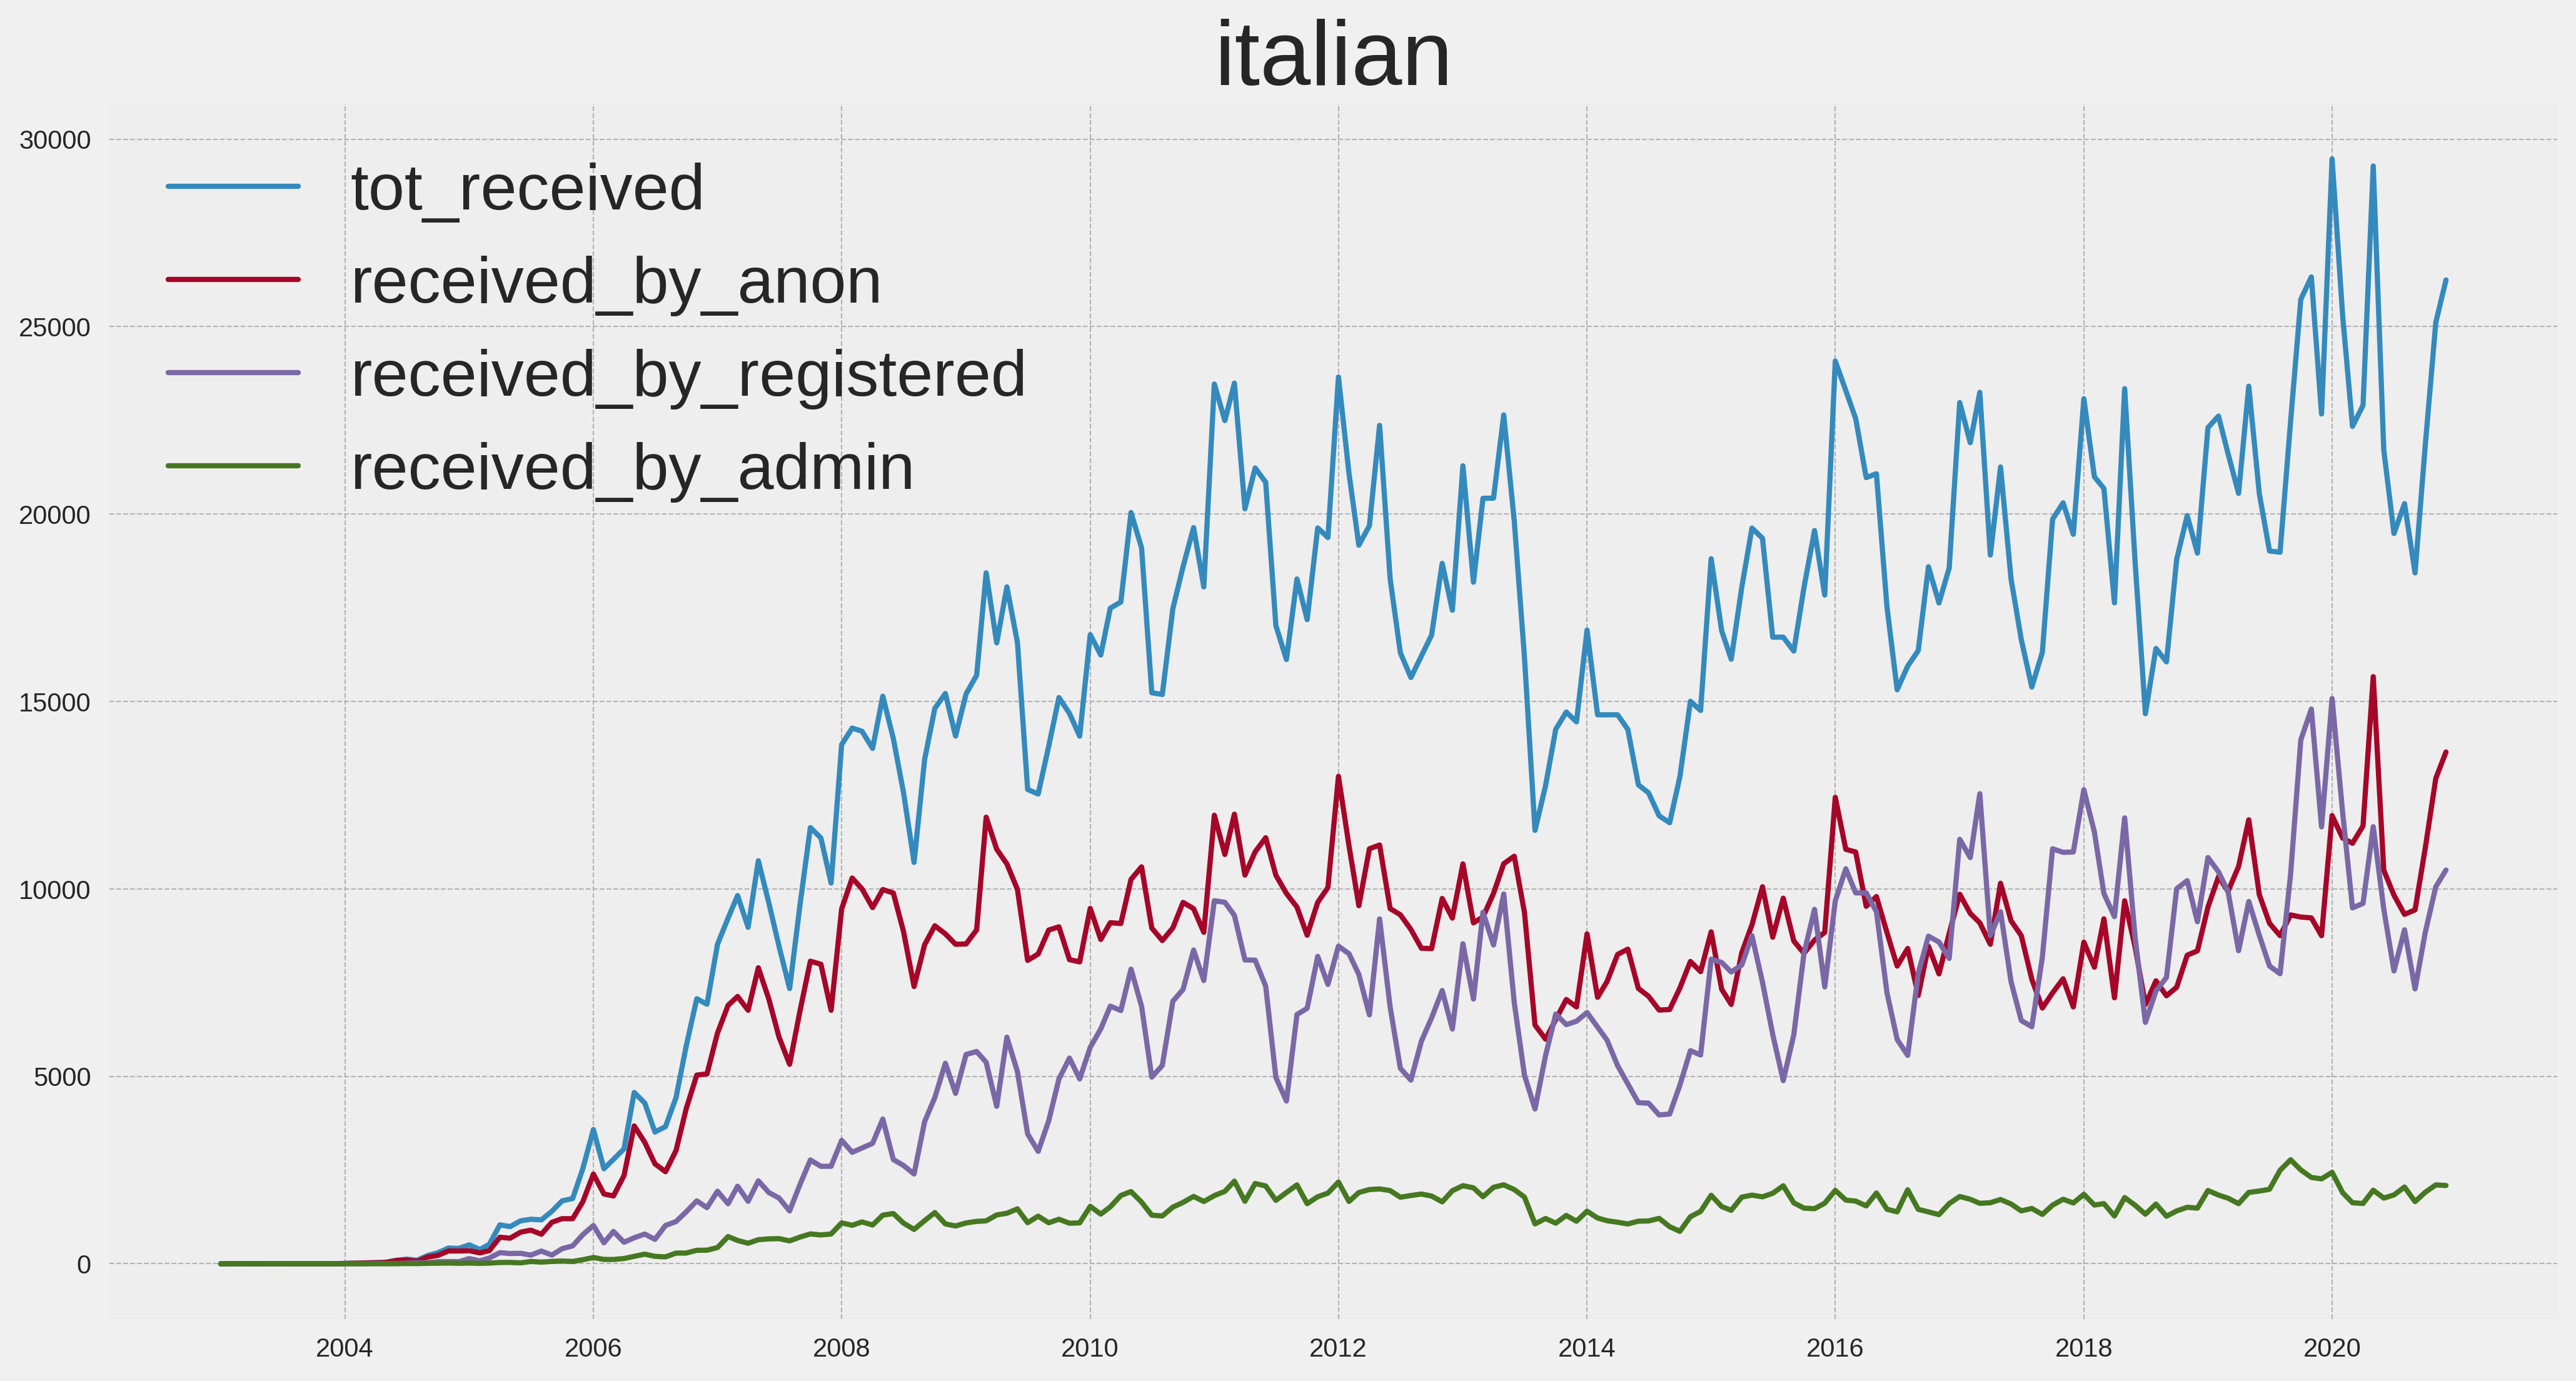
\includegraphics[width=0.49\textwidth]{./chapters/04/assets/revert_received_it.png}
    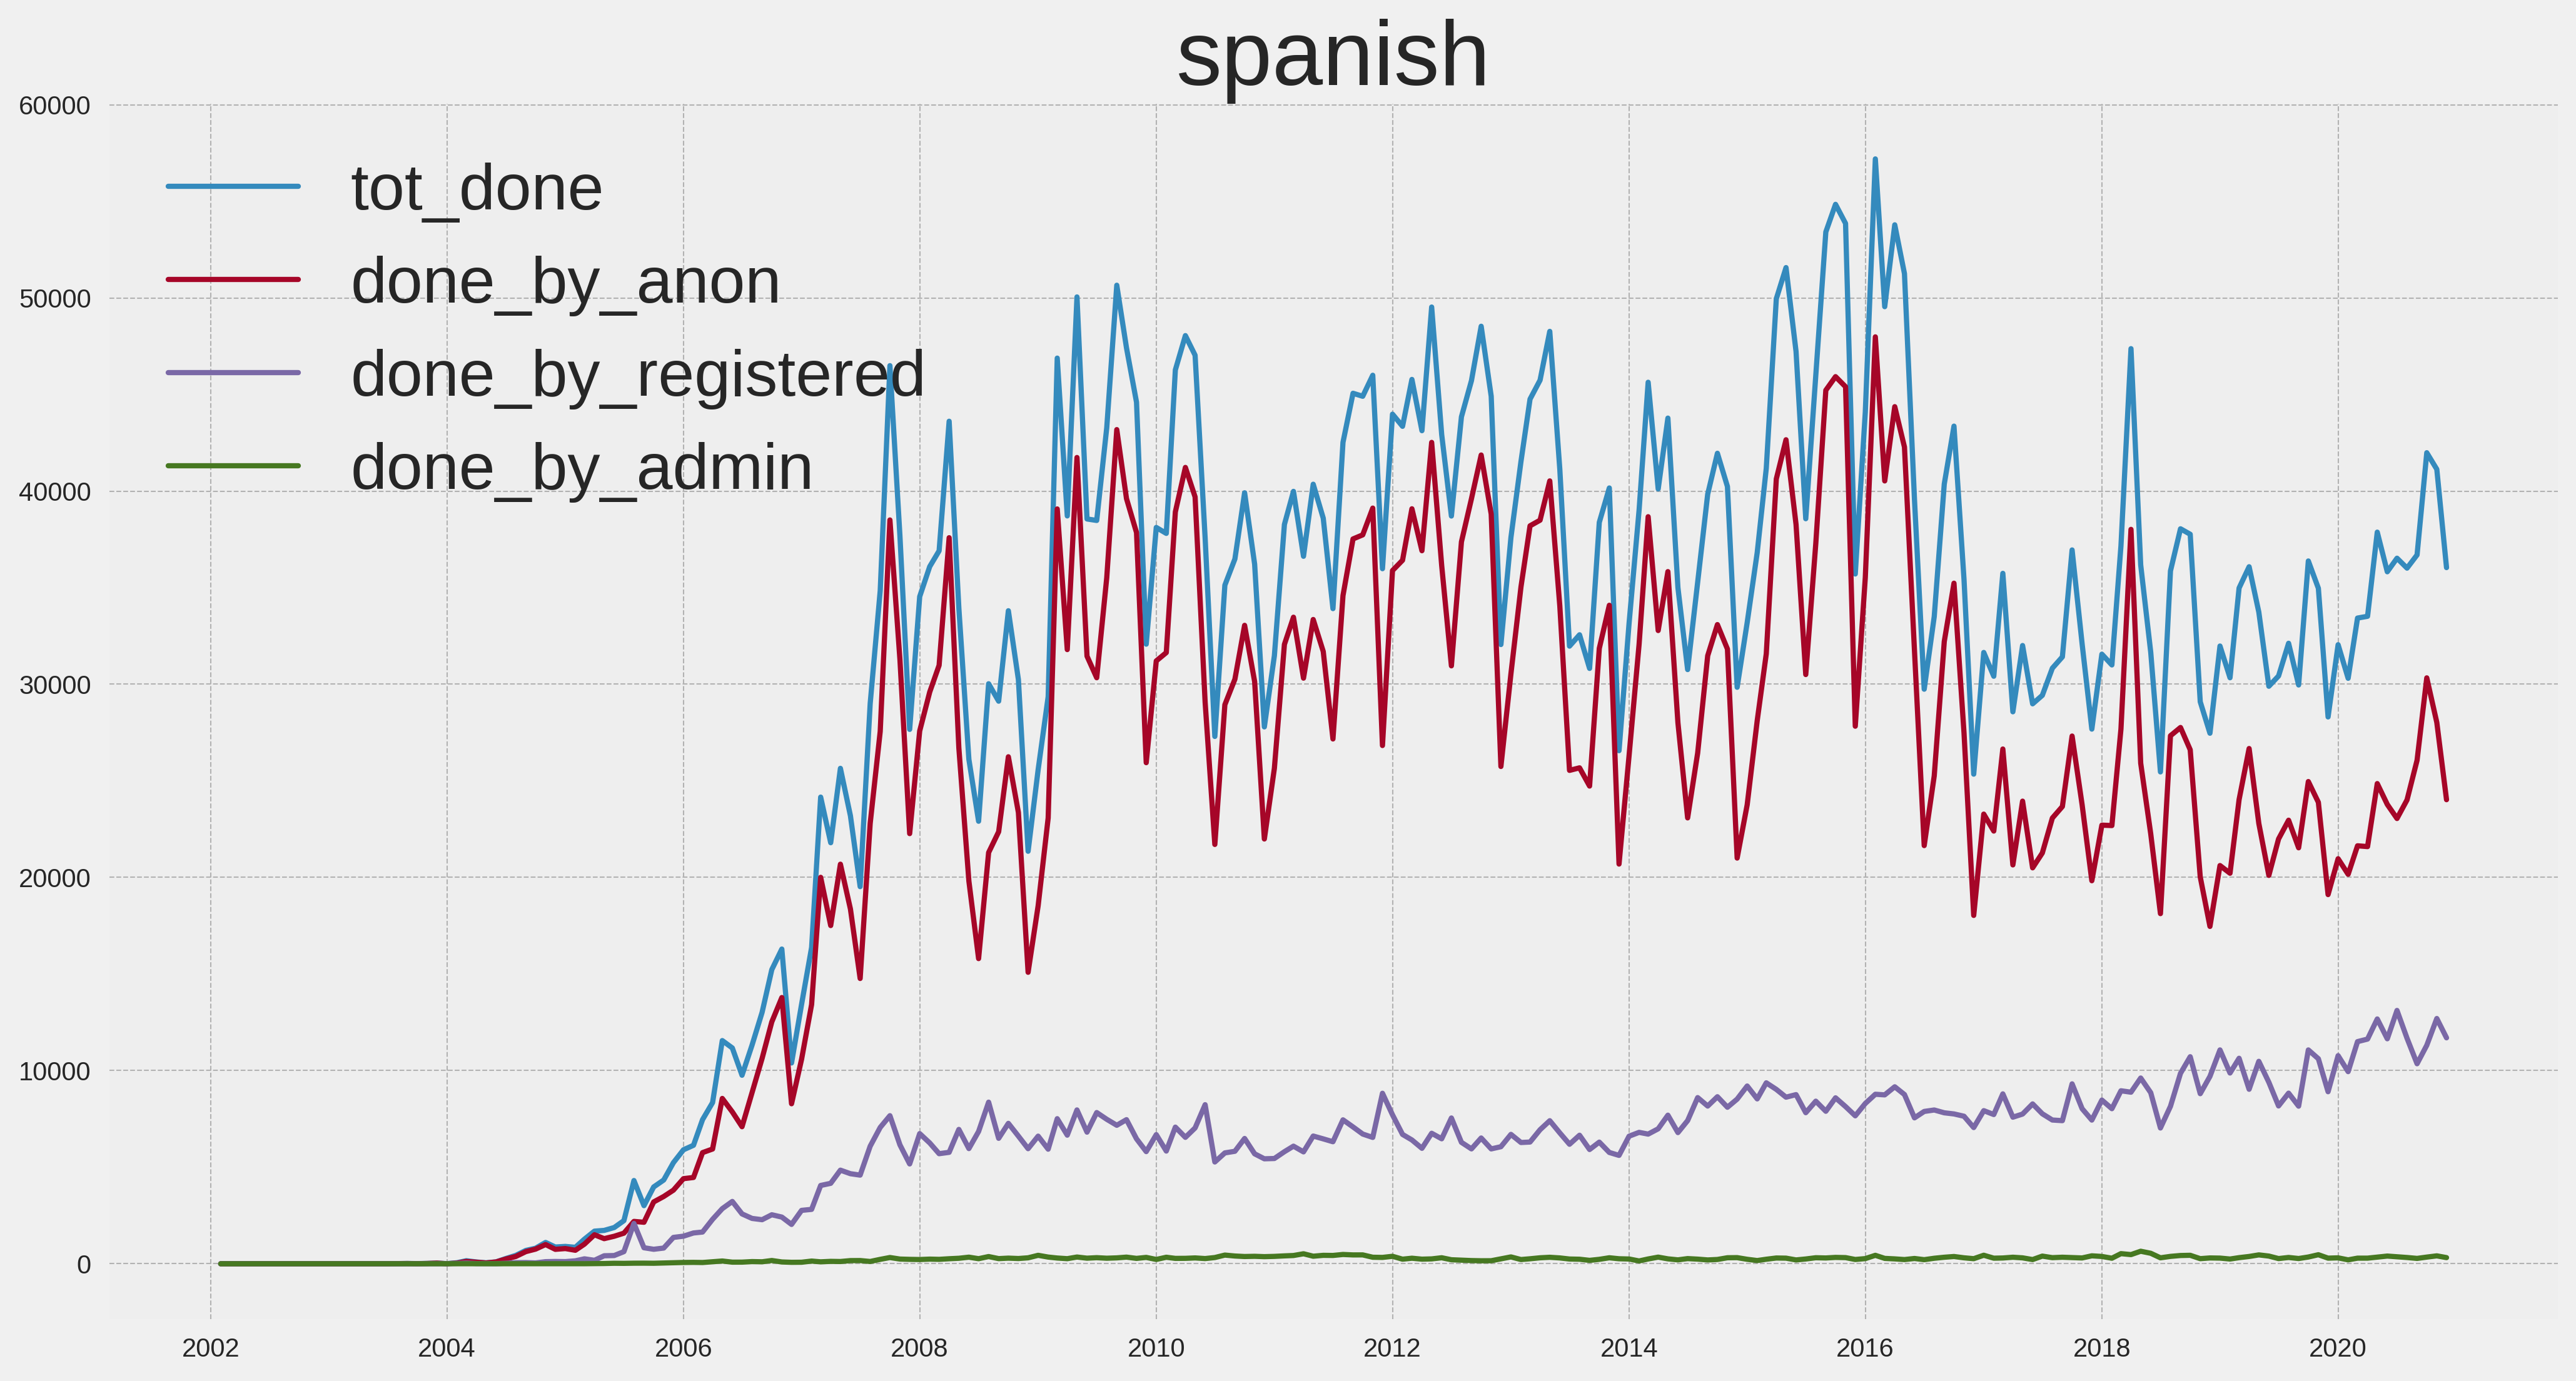
\includegraphics[width=0.49\textwidth]{./chapters/04/assets/revert_done_es.png}
    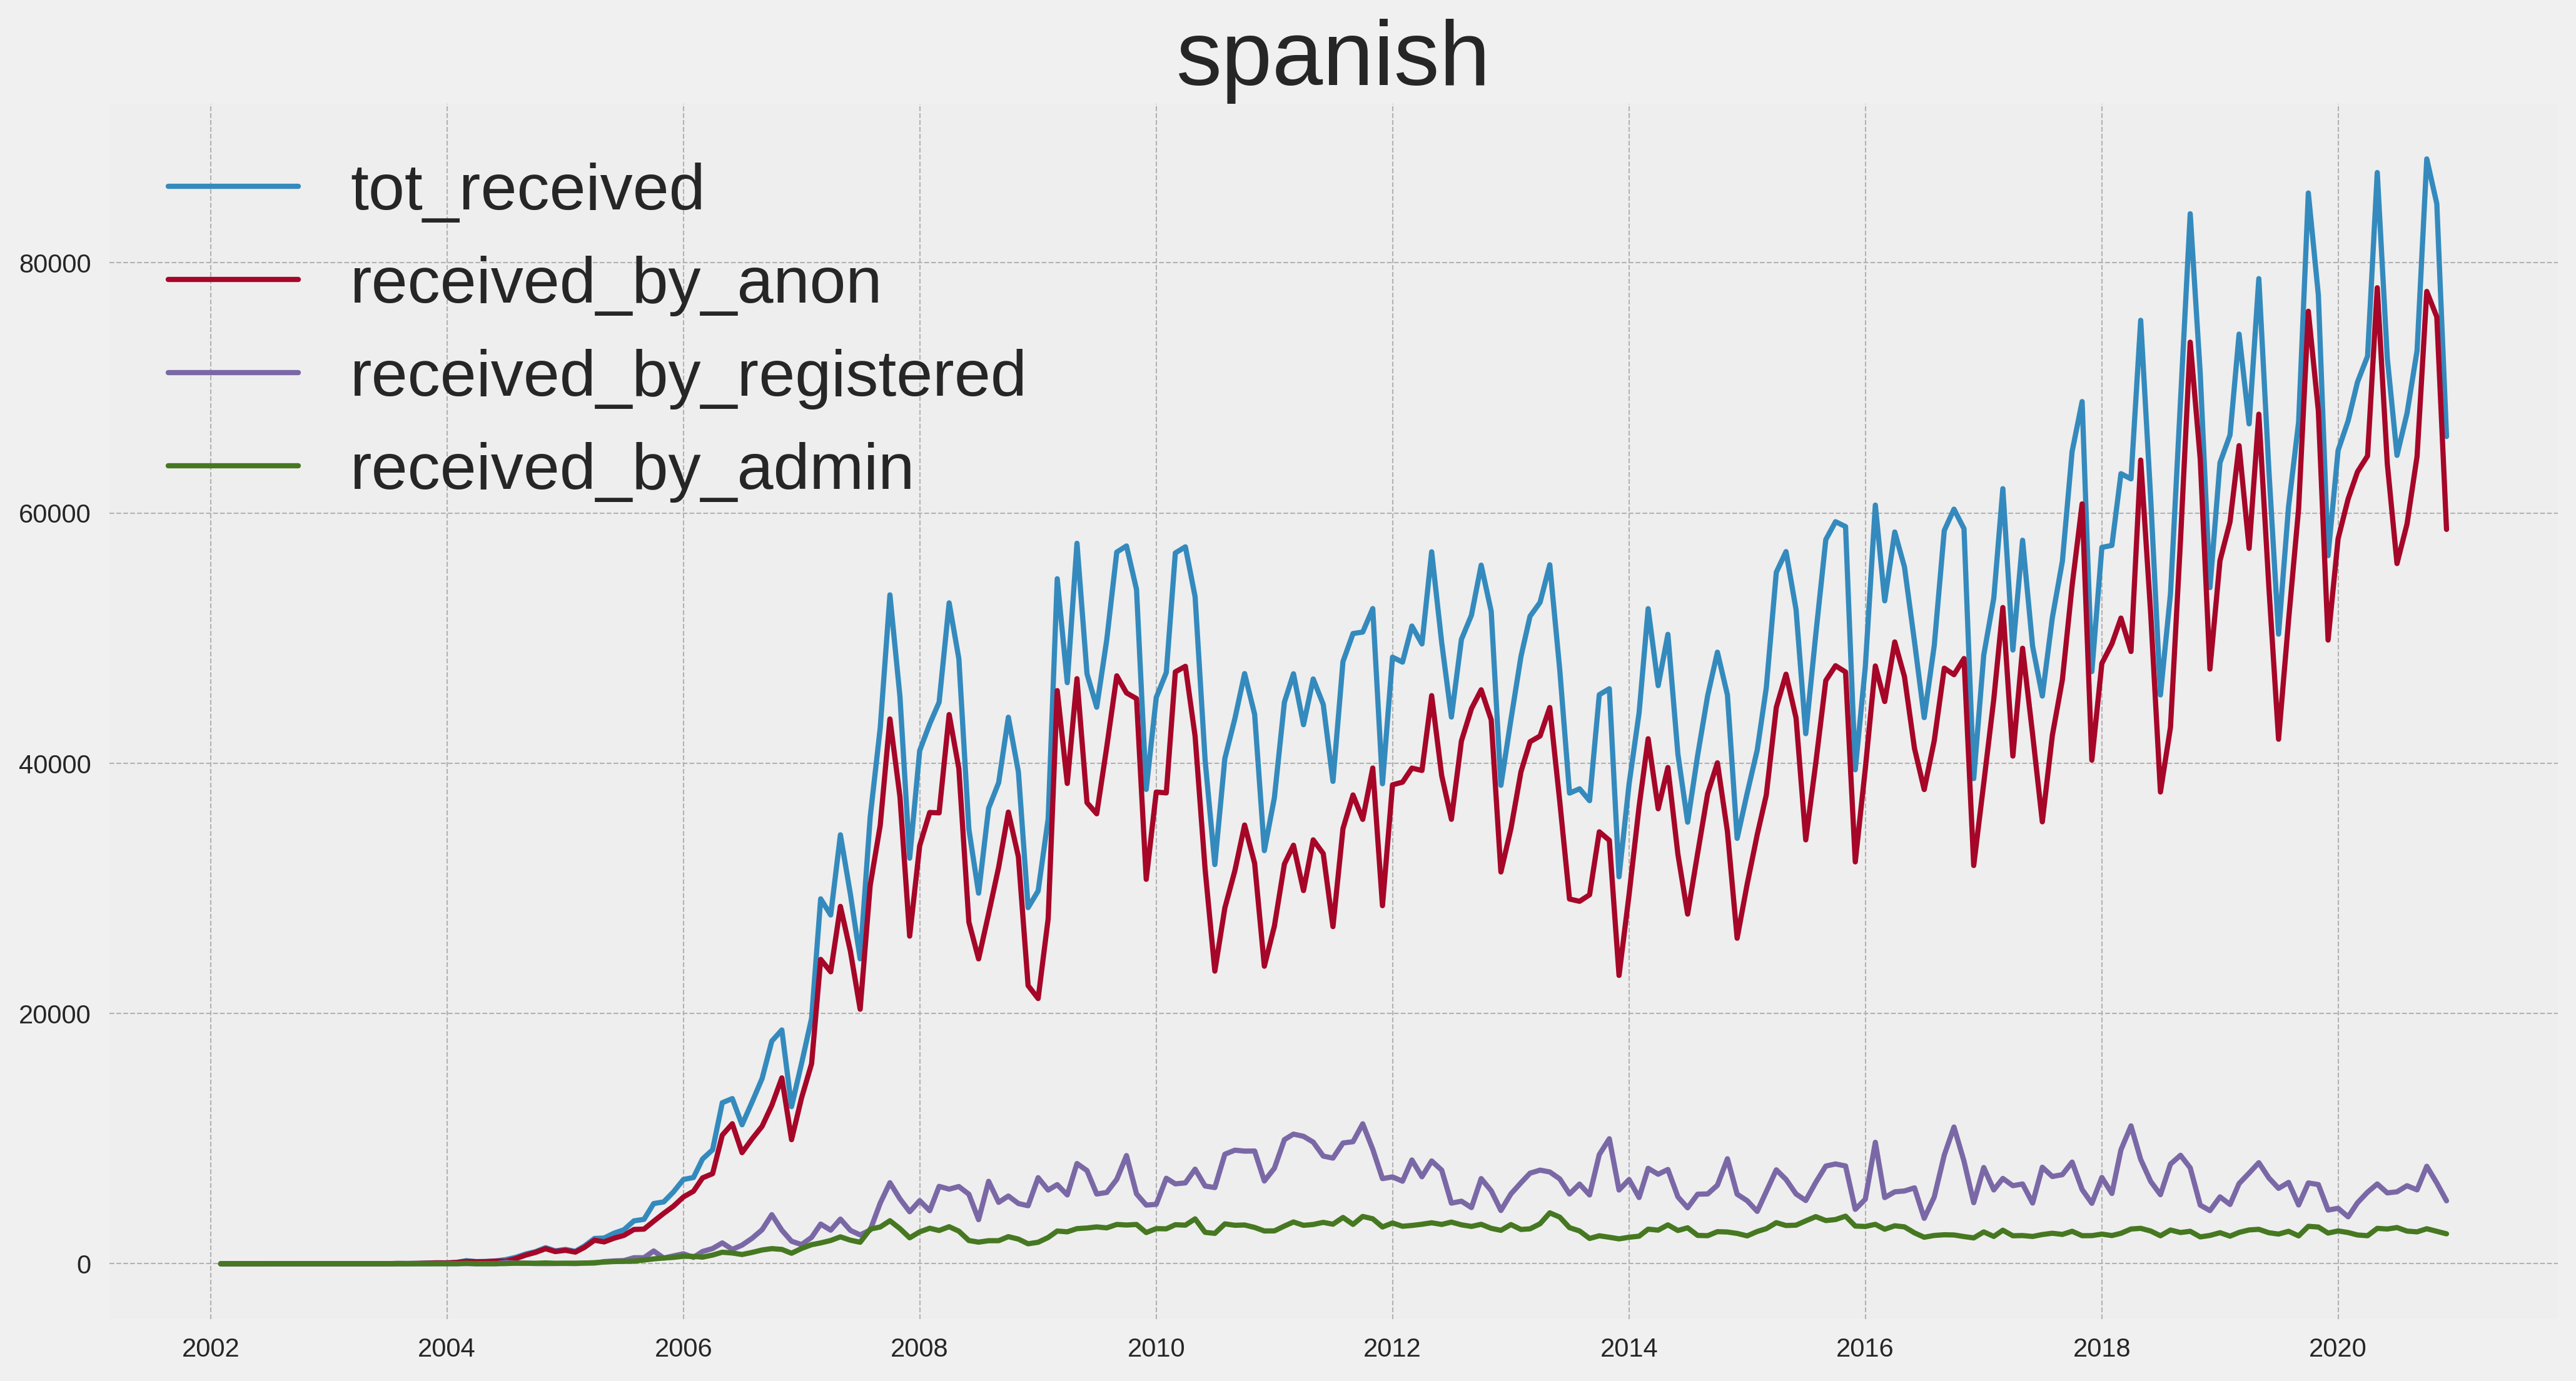
\includegraphics[width=0.49\textwidth]{./chapters/04/assets/revert_received_es.png}
    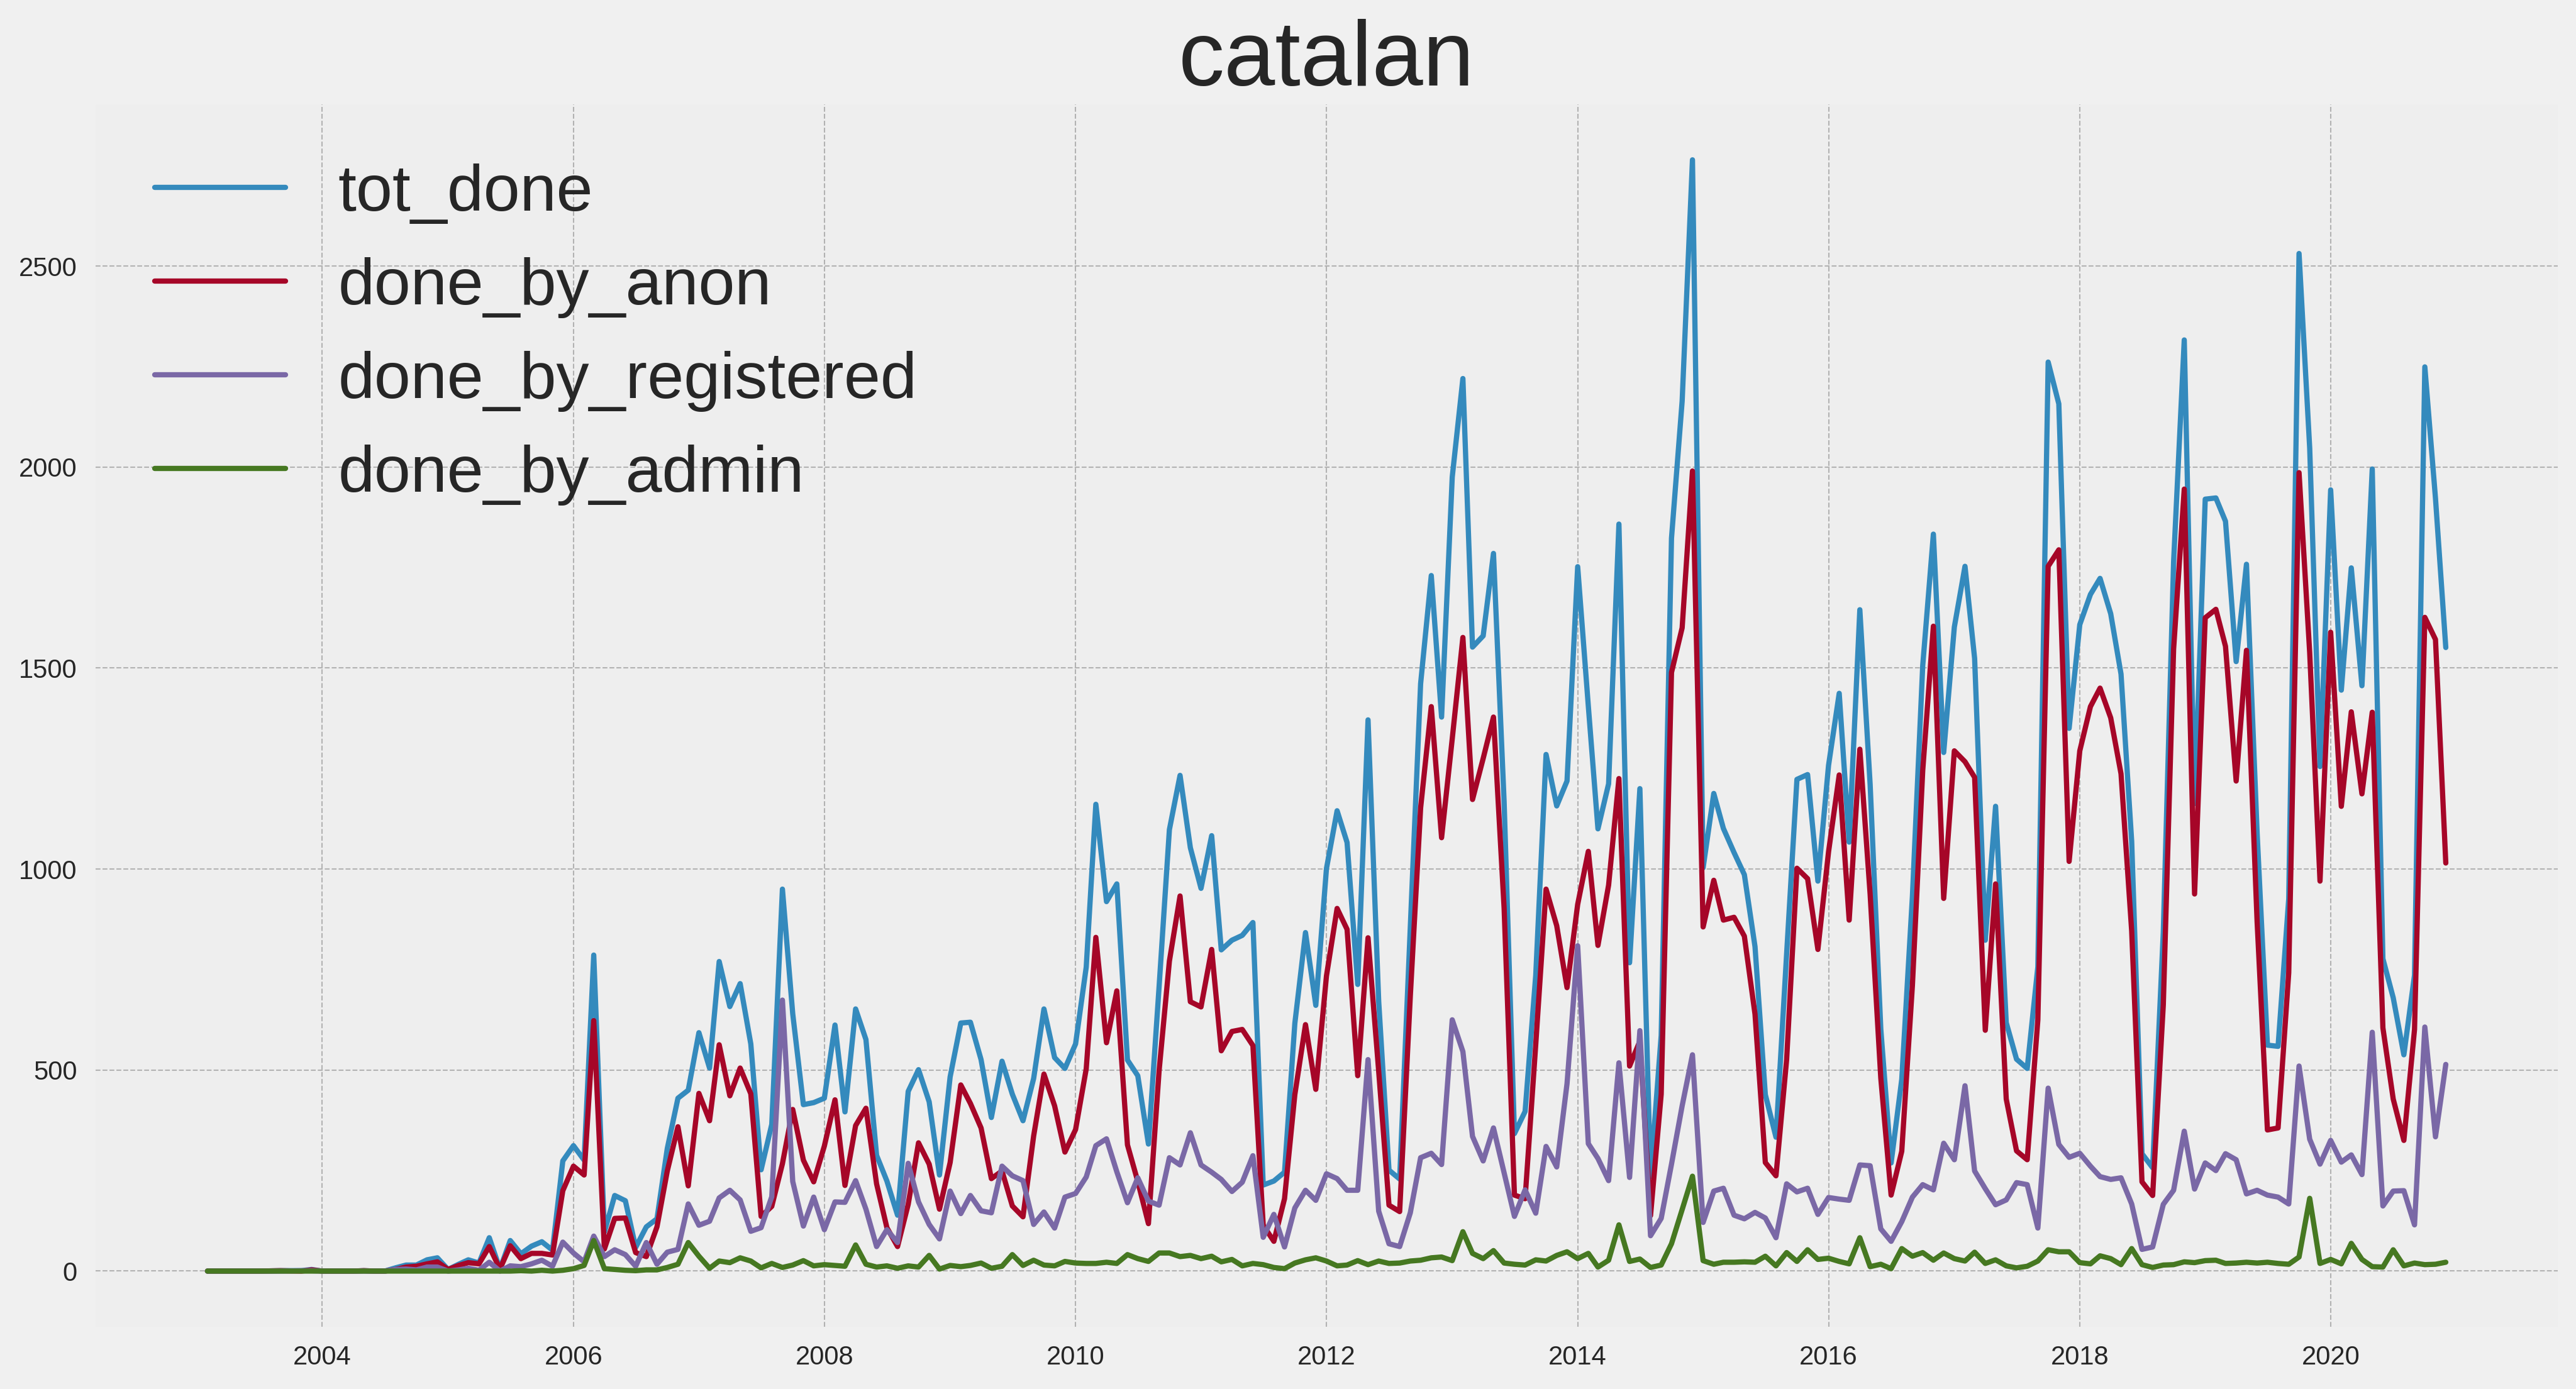
\includegraphics[width=0.49\textwidth]{./chapters/04/assets/revert_done_ca.png}
    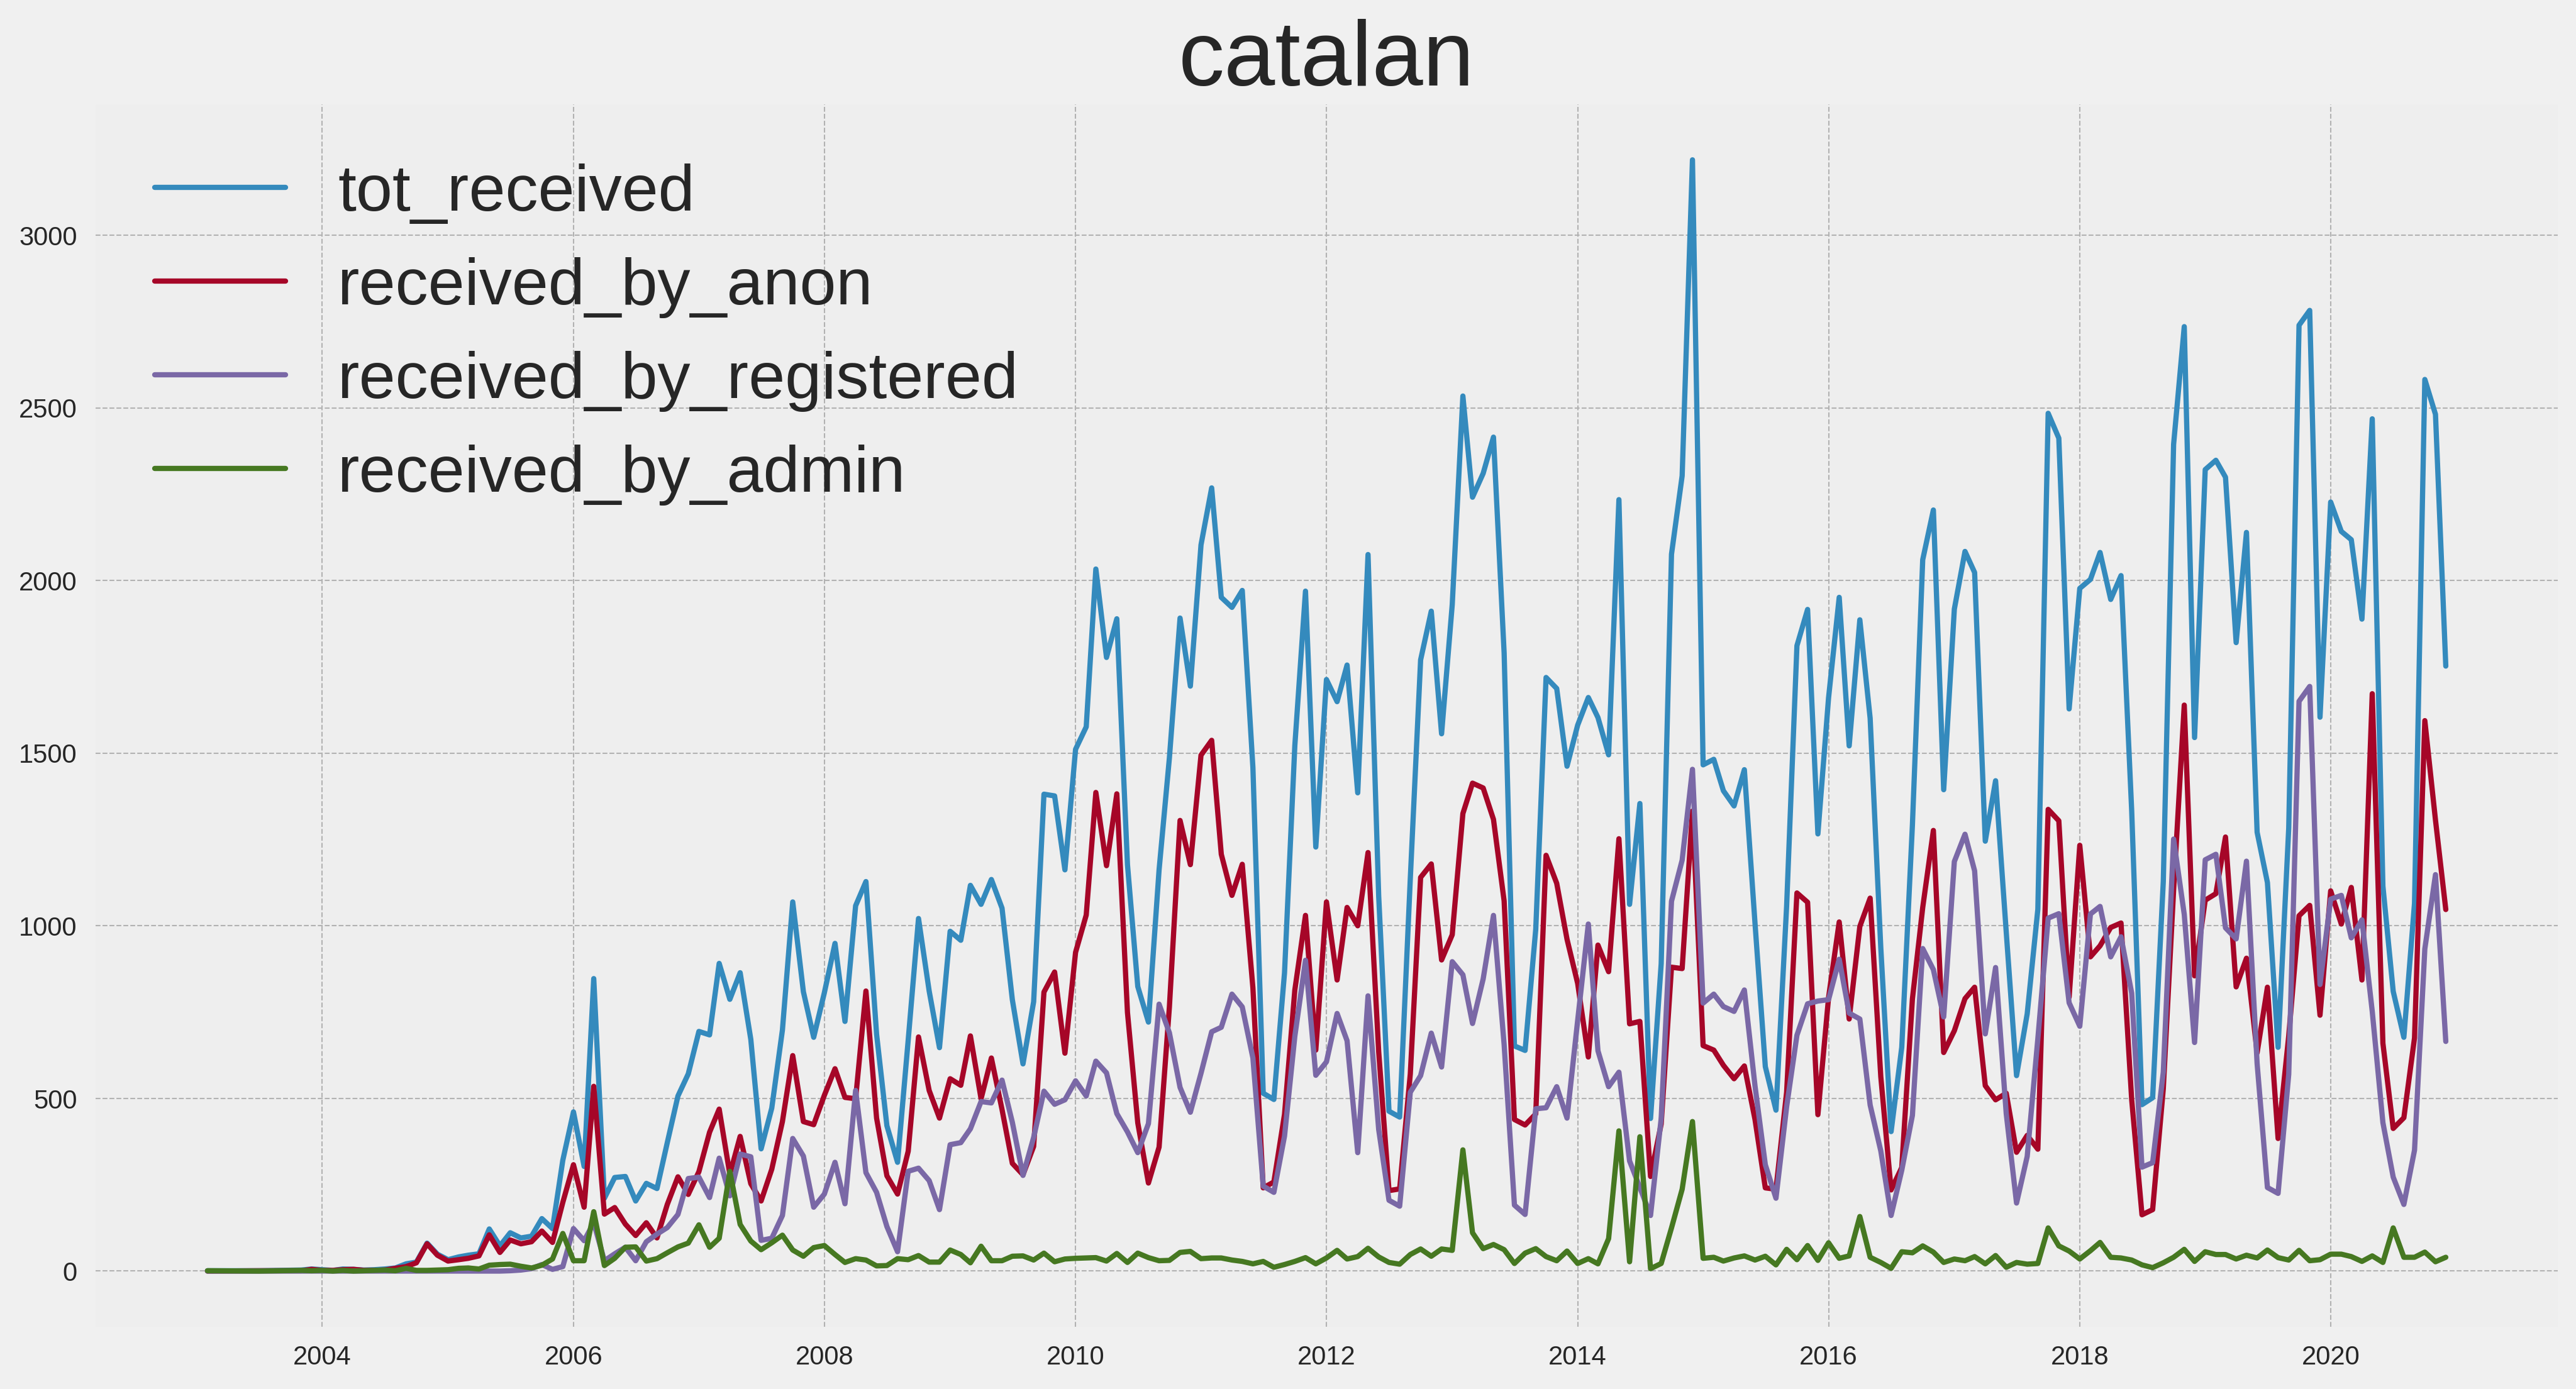
\includegraphics[width=0.49\textwidth]{./chapters/04/assets/revert_received_ca.png}
    \caption{Number of reverts made and received in Spanish, Italian, and Catalan Wikipedia divided by group.}
    \label{fig:revuser}
\end{figure}









